% Options for packages loaded elsewhere
\PassOptionsToPackage{unicode}{hyperref}
\PassOptionsToPackage{hyphens}{url}
%
\documentclass[
  man,floatsintext]{apa6}
\usepackage{amsmath,amssymb}
\usepackage{iftex}
\ifPDFTeX
  \usepackage[T1]{fontenc}
  \usepackage[utf8]{inputenc}
  \usepackage{textcomp} % provide euro and other symbols
\else % if luatex or xetex
  \usepackage{unicode-math} % this also loads fontspec
  \defaultfontfeatures{Scale=MatchLowercase}
  \defaultfontfeatures[\rmfamily]{Ligatures=TeX,Scale=1}
\fi
\usepackage{lmodern}
\ifPDFTeX\else
  % xetex/luatex font selection
\fi
% Use upquote if available, for straight quotes in verbatim environments
\IfFileExists{upquote.sty}{\usepackage{upquote}}{}
\IfFileExists{microtype.sty}{% use microtype if available
  \usepackage[]{microtype}
  \UseMicrotypeSet[protrusion]{basicmath} % disable protrusion for tt fonts
}{}
\makeatletter
\@ifundefined{KOMAClassName}{% if non-KOMA class
  \IfFileExists{parskip.sty}{%
    \usepackage{parskip}
  }{% else
    \setlength{\parindent}{0pt}
    \setlength{\parskip}{6pt plus 2pt minus 1pt}}
}{% if KOMA class
  \KOMAoptions{parskip=half}}
\makeatother
\usepackage{xcolor}
\usepackage{color}
\usepackage{fancyvrb}
\newcommand{\VerbBar}{|}
\newcommand{\VERB}{\Verb[commandchars=\\\{\}]}
\DefineVerbatimEnvironment{Highlighting}{Verbatim}{commandchars=\\\{\}}
% Add ',fontsize=\small' for more characters per line
\usepackage{framed}
\definecolor{shadecolor}{RGB}{248,248,248}
\newenvironment{Shaded}{\begin{snugshade}}{\end{snugshade}}
\newcommand{\AlertTok}[1]{\textcolor[rgb]{0.94,0.16,0.16}{#1}}
\newcommand{\AnnotationTok}[1]{\textcolor[rgb]{0.56,0.35,0.01}{\textbf{\textit{#1}}}}
\newcommand{\AttributeTok}[1]{\textcolor[rgb]{0.13,0.29,0.53}{#1}}
\newcommand{\BaseNTok}[1]{\textcolor[rgb]{0.00,0.00,0.81}{#1}}
\newcommand{\BuiltInTok}[1]{#1}
\newcommand{\CharTok}[1]{\textcolor[rgb]{0.31,0.60,0.02}{#1}}
\newcommand{\CommentTok}[1]{\textcolor[rgb]{0.56,0.35,0.01}{\textit{#1}}}
\newcommand{\CommentVarTok}[1]{\textcolor[rgb]{0.56,0.35,0.01}{\textbf{\textit{#1}}}}
\newcommand{\ConstantTok}[1]{\textcolor[rgb]{0.56,0.35,0.01}{#1}}
\newcommand{\ControlFlowTok}[1]{\textcolor[rgb]{0.13,0.29,0.53}{\textbf{#1}}}
\newcommand{\DataTypeTok}[1]{\textcolor[rgb]{0.13,0.29,0.53}{#1}}
\newcommand{\DecValTok}[1]{\textcolor[rgb]{0.00,0.00,0.81}{#1}}
\newcommand{\DocumentationTok}[1]{\textcolor[rgb]{0.56,0.35,0.01}{\textbf{\textit{#1}}}}
\newcommand{\ErrorTok}[1]{\textcolor[rgb]{0.64,0.00,0.00}{\textbf{#1}}}
\newcommand{\ExtensionTok}[1]{#1}
\newcommand{\FloatTok}[1]{\textcolor[rgb]{0.00,0.00,0.81}{#1}}
\newcommand{\FunctionTok}[1]{\textcolor[rgb]{0.13,0.29,0.53}{\textbf{#1}}}
\newcommand{\ImportTok}[1]{#1}
\newcommand{\InformationTok}[1]{\textcolor[rgb]{0.56,0.35,0.01}{\textbf{\textit{#1}}}}
\newcommand{\KeywordTok}[1]{\textcolor[rgb]{0.13,0.29,0.53}{\textbf{#1}}}
\newcommand{\NormalTok}[1]{#1}
\newcommand{\OperatorTok}[1]{\textcolor[rgb]{0.81,0.36,0.00}{\textbf{#1}}}
\newcommand{\OtherTok}[1]{\textcolor[rgb]{0.56,0.35,0.01}{#1}}
\newcommand{\PreprocessorTok}[1]{\textcolor[rgb]{0.56,0.35,0.01}{\textit{#1}}}
\newcommand{\RegionMarkerTok}[1]{#1}
\newcommand{\SpecialCharTok}[1]{\textcolor[rgb]{0.81,0.36,0.00}{\textbf{#1}}}
\newcommand{\SpecialStringTok}[1]{\textcolor[rgb]{0.31,0.60,0.02}{#1}}
\newcommand{\StringTok}[1]{\textcolor[rgb]{0.31,0.60,0.02}{#1}}
\newcommand{\VariableTok}[1]{\textcolor[rgb]{0.00,0.00,0.00}{#1}}
\newcommand{\VerbatimStringTok}[1]{\textcolor[rgb]{0.31,0.60,0.02}{#1}}
\newcommand{\WarningTok}[1]{\textcolor[rgb]{0.56,0.35,0.01}{\textbf{\textit{#1}}}}
\usepackage{graphicx}
\makeatletter
\def\maxwidth{\ifdim\Gin@nat@width>\linewidth\linewidth\else\Gin@nat@width\fi}
\def\maxheight{\ifdim\Gin@nat@height>\textheight\textheight\else\Gin@nat@height\fi}
\makeatother
% Scale images if necessary, so that they will not overflow the page
% margins by default, and it is still possible to overwrite the defaults
% using explicit options in \includegraphics[width, height, ...]{}
\setkeys{Gin}{width=\maxwidth,height=\maxheight,keepaspectratio}
% Set default figure placement to htbp
\makeatletter
\def\fps@figure{htbp}
\makeatother
\setlength{\emergencystretch}{3em} % prevent overfull lines
\providecommand{\tightlist}{%
  \setlength{\itemsep}{0pt}\setlength{\parskip}{0pt}}
\setcounter{secnumdepth}{-\maxdimen} % remove section numbering
% Make \paragraph and \subparagraph free-standing
\ifx\paragraph\undefined\else
  \let\oldparagraph\paragraph
  \renewcommand{\paragraph}[1]{\oldparagraph{#1}\mbox{}}
\fi
\ifx\subparagraph\undefined\else
  \let\oldsubparagraph\subparagraph
  \renewcommand{\subparagraph}[1]{\oldsubparagraph{#1}\mbox{}}
\fi
% definitions for citeproc citations
\NewDocumentCommand\citeproctext{}{}
\NewDocumentCommand\citeproc{mm}{%
  \begingroup\def\citeproctext{#2}\cite{#1}\endgroup}
\makeatletter
 % allow citations to break across lines
 \let\@cite@ofmt\@firstofone
 % avoid brackets around text for \cite:
 \def\@biblabel#1{}
 \def\@cite#1#2{{#1\if@tempswa , #2\fi}}
\makeatother
\newlength{\cslhangindent}
\setlength{\cslhangindent}{1.5em}
\newlength{\csllabelwidth}
\setlength{\csllabelwidth}{3em}
\newenvironment{CSLReferences}[2] % #1 hanging-indent, #2 entry-spacing
 {\begin{list}{}{%
  \setlength{\itemindent}{0pt}
  \setlength{\leftmargin}{0pt}
  \setlength{\parsep}{0pt}
  % turn on hanging indent if param 1 is 1
  \ifodd #1
   \setlength{\leftmargin}{\cslhangindent}
   \setlength{\itemindent}{-1\cslhangindent}
  \fi
  % set entry spacing
  \setlength{\itemsep}{#2\baselineskip}}}
 {\end{list}}
\usepackage{calc}
\newcommand{\CSLBlock}[1]{\hfill\break\parbox[t]{\linewidth}{\strut\ignorespaces#1\strut}}
\newcommand{\CSLLeftMargin}[1]{\parbox[t]{\csllabelwidth}{\strut#1\strut}}
\newcommand{\CSLRightInline}[1]{\parbox[t]{\linewidth - \csllabelwidth}{\strut#1\strut}}
\newcommand{\CSLIndent}[1]{\hspace{\cslhangindent}#1}
\ifLuaTeX
\usepackage[bidi=basic]{babel}
\else
\usepackage[bidi=default]{babel}
\fi
\babelprovide[main,import]{english}
% get rid of language-specific shorthands (see #6817):
\let\LanguageShortHands\languageshorthands
\def\languageshorthands#1{}
% Manuscript styling
\usepackage{upgreek}
\captionsetup{font=singlespacing,justification=justified}

% Table formatting
\usepackage{longtable}
\usepackage{lscape}
% \usepackage[counterclockwise]{rotating}   % Landscape page setup for large tables
\usepackage{multirow}		% Table styling
\usepackage{tabularx}		% Control Column width
\usepackage[flushleft]{threeparttable}	% Allows for three part tables with a specified notes section
\usepackage{threeparttablex}            % Lets threeparttable work with longtable

% Create new environments so endfloat can handle them
% \newenvironment{ltable}
%   {\begin{landscape}\centering\begin{threeparttable}}
%   {\end{threeparttable}\end{landscape}}
\newenvironment{lltable}{\begin{landscape}\centering\begin{ThreePartTable}}{\end{ThreePartTable}\end{landscape}}

% Enables adjusting longtable caption width to table width
% Solution found at http://golatex.de/longtable-mit-caption-so-breit-wie-die-tabelle-t15767.html
\makeatletter
\newcommand\LastLTentrywidth{1em}
\newlength\longtablewidth
\setlength{\longtablewidth}{1in}
\newcommand{\getlongtablewidth}{\begingroup \ifcsname LT@\roman{LT@tables}\endcsname \global\longtablewidth=0pt \renewcommand{\LT@entry}[2]{\global\advance\longtablewidth by ##2\relax\gdef\LastLTentrywidth{##2}}\@nameuse{LT@\roman{LT@tables}} \fi \endgroup}

% \setlength{\parindent}{0.5in}
% \setlength{\parskip}{0pt plus 0pt minus 0pt}

% Overwrite redefinition of paragraph and subparagraph by the default LaTeX template
% See https://github.com/crsh/papaja/issues/292
\makeatletter
\renewcommand{\paragraph}{\@startsection{paragraph}{4}{\parindent}%
  {0\baselineskip \@plus 0.2ex \@minus 0.2ex}%
  {-1em}%
  {\normalfont\normalsize\bfseries\itshape\typesectitle}}

\renewcommand{\subparagraph}[1]{\@startsection{subparagraph}{5}{1em}%
  {0\baselineskip \@plus 0.2ex \@minus 0.2ex}%
  {-\z@\relax}%
  {\normalfont\normalsize\itshape\hspace{\parindent}{#1}\textit{\addperi}}{\relax}}
\makeatother

% \usepackage{etoolbox}
\makeatletter
\patchcmd{\HyOrg@maketitle}
  {\section{\normalfont\normalsize\abstractname}}
  {\section*{\normalfont\normalsize\abstractname}}
  {}{\typeout{Failed to patch abstract.}}
\patchcmd{\HyOrg@maketitle}
  {\section{\protect\normalfont{\@title}}}
  {\section*{\protect\normalfont{\@title}}}
  {}{\typeout{Failed to patch title.}}
\makeatother

\usepackage{xpatch}
\makeatletter
\xapptocmd\appendix
  {\xapptocmd\section
    {\addcontentsline{toc}{section}{\appendixname\ifoneappendix\else~\theappendix\fi\\: #1}}
    {}{\InnerPatchFailed}%
  }
{}{\PatchFailed}
\usepackage{csquotes}
\usepackage{amsmath}
\usepackage{tikz}
\usetikzlibrary{shapes.geometric,arrows, positioning}
\usepackage[LGRgreek]{mathastext}
\ifLuaTeX
  \usepackage{selnolig}  % disable illegal ligatures
\fi
\usepackage{bookmark}
\IfFileExists{xurl.sty}{\usepackage{xurl}}{} % add URL line breaks if available
\urlstyle{same}
\hypersetup{
  pdftitle={Visual Partitions},
  pdfauthor={Dustin A. Fife1},
  pdflang={en-EN},
  hidelinks,
  pdfcreator={LaTeX via pandoc}}

\title{Visual Partitions}
\author{Dustin A. Fife\textsuperscript{1}}
\date{}


\shorttitle{Visual Partitions}

\authornote{

Correspondence concerning this article should be addressed to Dustin A. Fife, 201 Mullica Hill Road Glassboro, NJ 08028. E-mail: \href{mailto:fife.dustin@gmail.com}{\nolinkurl{fife.dustin@gmail.com}}

}

\affiliation{\vspace{0.5cm}\textsuperscript{1} Rowan University}

\abstract{%
Researchers routinely utilize multiple predictor variables and summarize their results using ANOVA summary (or regression) tables. These tables are relatively uninformative and often misleading. They fail to show the nature of main effects (e.g., size and direction) and interaction effects, and they also make it hard to assess the viability of the statistical model. A better approach is to use what I call ``visual partitions,'' which are intuitive, succinct visual representations of the statistical model. By leveraging our advanced visual pattern recognition system, these visual partitions provide digestible, informative summaries of statistical models. These partitions (and the rules associated with them) allow us to identify when effects can be partitioned into relatively independent visual representations. In this paper, I highlight when conditional inferences are contaminated by other features of the model and identify the conditions under which effects can be partitioned. I also reveal a strategy for partitioning effects into uncontaminated blocks using visualizations. This approach simplifies analyses immensely, without oversimplifying the analysis.
}



\begin{document}
\maketitle

\section{Introduction}\label{introduction}

Suppose we were to peruse our favorite journal and find the results shown in Table \ref{tab:anovatab}. This table presents the results of a model where suicide ideation is modeled from stress, health, depression, and the suicide ideation of one's best friend. Further suppose these results are highly related to our area of expertise. As such, we have great interest in understanding how these variables relate to suicide ideation. How are we to make sense of these results? Does increasing health reduce suicide ideation? Or does it increase it? How about stress? The model suggests a nonlinear effect between stress and suicide ideation, but what is the nature of that effect? And what of the interaction? In what way do friend ideation and depression interact?

\begin{table}[tbp]

\begin{center}
\begin{threeparttable}

\caption{\label{tab:anovatab}ANOVA Summary Table of the Suicide Ideation Analysis}

\begin{tabular}{lccccc}
\toprule
 & DF & SS & MS & F & p\\
\midrule
stress & 1 & 1,598.37 & 1,598.37 & 874.68 & <0.001\\
$\text{stress}^2$ & 1 & 8,374.25 & 8,374.25 & 4582.65 & <0.001\\
health & 1 & 2,097.66 & 2,097.66 & 1147.9 & <0.001\\
friend ideation & 1 & 699.67 & 699.67 & 382.88 & <0.001\\
depression & 1 & 5,797.63 & 5,797.63 & 3172.64 & <0.001\\
friend ideation $ \times $ depression & 1 & 2,954.06 & 2,954.06 & 1616.55 & <0.001\\
Residuals & 2993 & 5,469.36 & 1.83 &  & \\
\bottomrule
\end{tabular}

\end{threeparttable}
\end{center}

\end{table}

Unfortunately, an ANOVA summary table cannot answer these questions. Regression tables are slightly better because they convey the size/direction of an effect, but such tables are still painfully uninformative. Even if we were to know the direction of the main effects and the nature of the interaction/nonlinear effects, there's still the multivariate nature of the data to content with.\footnote{Technically, the term ``multivariate'' means there are multiple \emph{dependent} variables. However, the term is frequently (mis)used to describe situations where multiple \emph{independent} variables are used. The latter situation is generally referred to as ``multiple regression.'' However, that too is easy to misunderstand, since many assume multiple regression is used only when one has multiple numeric predictors (Cohen, 1968). This is incorrect; multiple regression can be used to model categorical predictors. As such multiple regression subsumes factorial ANOVAs and ANCOVAs. However, in this paper, I adopt the nomenclature of nonstatisticians since it is arguably more common. As such, I use the term ``multivariate'' to refer to situations where the researcher has multiple independent variables.} These predictors were fit in one multivariate model. Can we interpret the main effects in isolation? If not, how do we interpret main effects multivariately? And what of the nonlinear effects? In short, how do we interpret the whole of the multivariate model without introducing bias in our interpretation?

It turns out, the answer to that question is quite simple and requires the use of simple visualizations I call ``visual partitions.'' Visual partitions leverage our advanced pattern recognition system (Otten, Cheng, \& Drewnowski, 2015), making it far easier to interpret a statistical model than with a table of results. These visual partitions are supplements (or, perhaps, replacements) of the traditional ANOVA summary table for summarizing the results of a study. Visual partitions succinctly communicate the \emph{entirety} of a multivariate model without introducing bias in interpretation. This approach helps identify which effects can be interpreted in independent visuals and which must be interpreted together.

However, before introducing the visual partitions approach, I must introduce several visualization tools we will use throughout this manuscript. Subsequently, I will identify the rules and assumptions required to create visual partitions. Next, I show how visual partitions can be used for confirmatory research, then introduce a strategy for using visual partitions in exploratory research. I then conclude with an example and show how a visual partitions approach helps detect insights that would have been missed with traditional approaches.

\section{Visualization Tools}\label{visualization-tools}

One critical component of the visual partitioning strategy is plotting nonlinear and/or interactive effects. (The reason these are critical will be explained in the following section). Visualizing nonlinear relationships is simple; one simply needs to utilize a scatterplot and (optionally) overlay a nonlinear line (e.g., quadratic, cubic spline, or loess line).

There are also many tools to visualize interaction effects. One approach is a ``simple-slopes'' analysis (Cohen, Cohen, West, \& Aiken, 2013), where the user picks a few relatively arbitrary points on the moderator (e.g., +1 SD, mean, and -1 SD), then shows the regression lines for the other predictor variable at each of these levels of the moderator. While this approach is both intuitive and easy to perform, it suffers from several weaknesses: the points chosen (i.e., \(\pm\) 1 SD/mean) may occur where data are quite sparse (Finsaas \& Goldstein, 2020); these plots do not show raw data, which makes it harder to assess model assumptions (McCabe, Kim, \& King, 2018); and the choice of which predictor variable is considered the moderator is arbitrary (Finsaas \& Goldstein, 2020). Scholars have proposed alternative methods, including 3-D planes (Cohen et al., 2013; Finsaas \& Goldstein, 2020), the Johnson-Neyman technique (Bauer, 2005; Finsaas \& Goldstein, 2020; Johnson \& Neyman, 1936), and paneled plots (McCabe et al., 2018). Most of these methods are effective for the purposes for which they were designed, while many will not serve the purposes of this paper. For this paper, I will utilize three important tools: Flexplot, marginal plots, and partial residual plots. These graphical tools show raw data, are easy to interpret, and respect the multivariate nature of the data. I will discuss each of these in turn.

\subsection{Tool \#1: Flexplot}\label{tool-1-flexplot}

The first tool I will utilize is Flexplot (Fife, 2021). Flexplot was designed to provide an easy-to-use interface for statistical modeling. With one-line functions, users can visualize univariate, bivariate, and multivariate relationships. Flexplot is available as an R package (see Fife, 2021), as well as a point-and-click interface in both JASP {[}JASP Team (2019); fife2021graph{]} and Jamovi {[}The Jamovi Project (2019); Fife2019c{]}.

\begin{figure}

{\centering 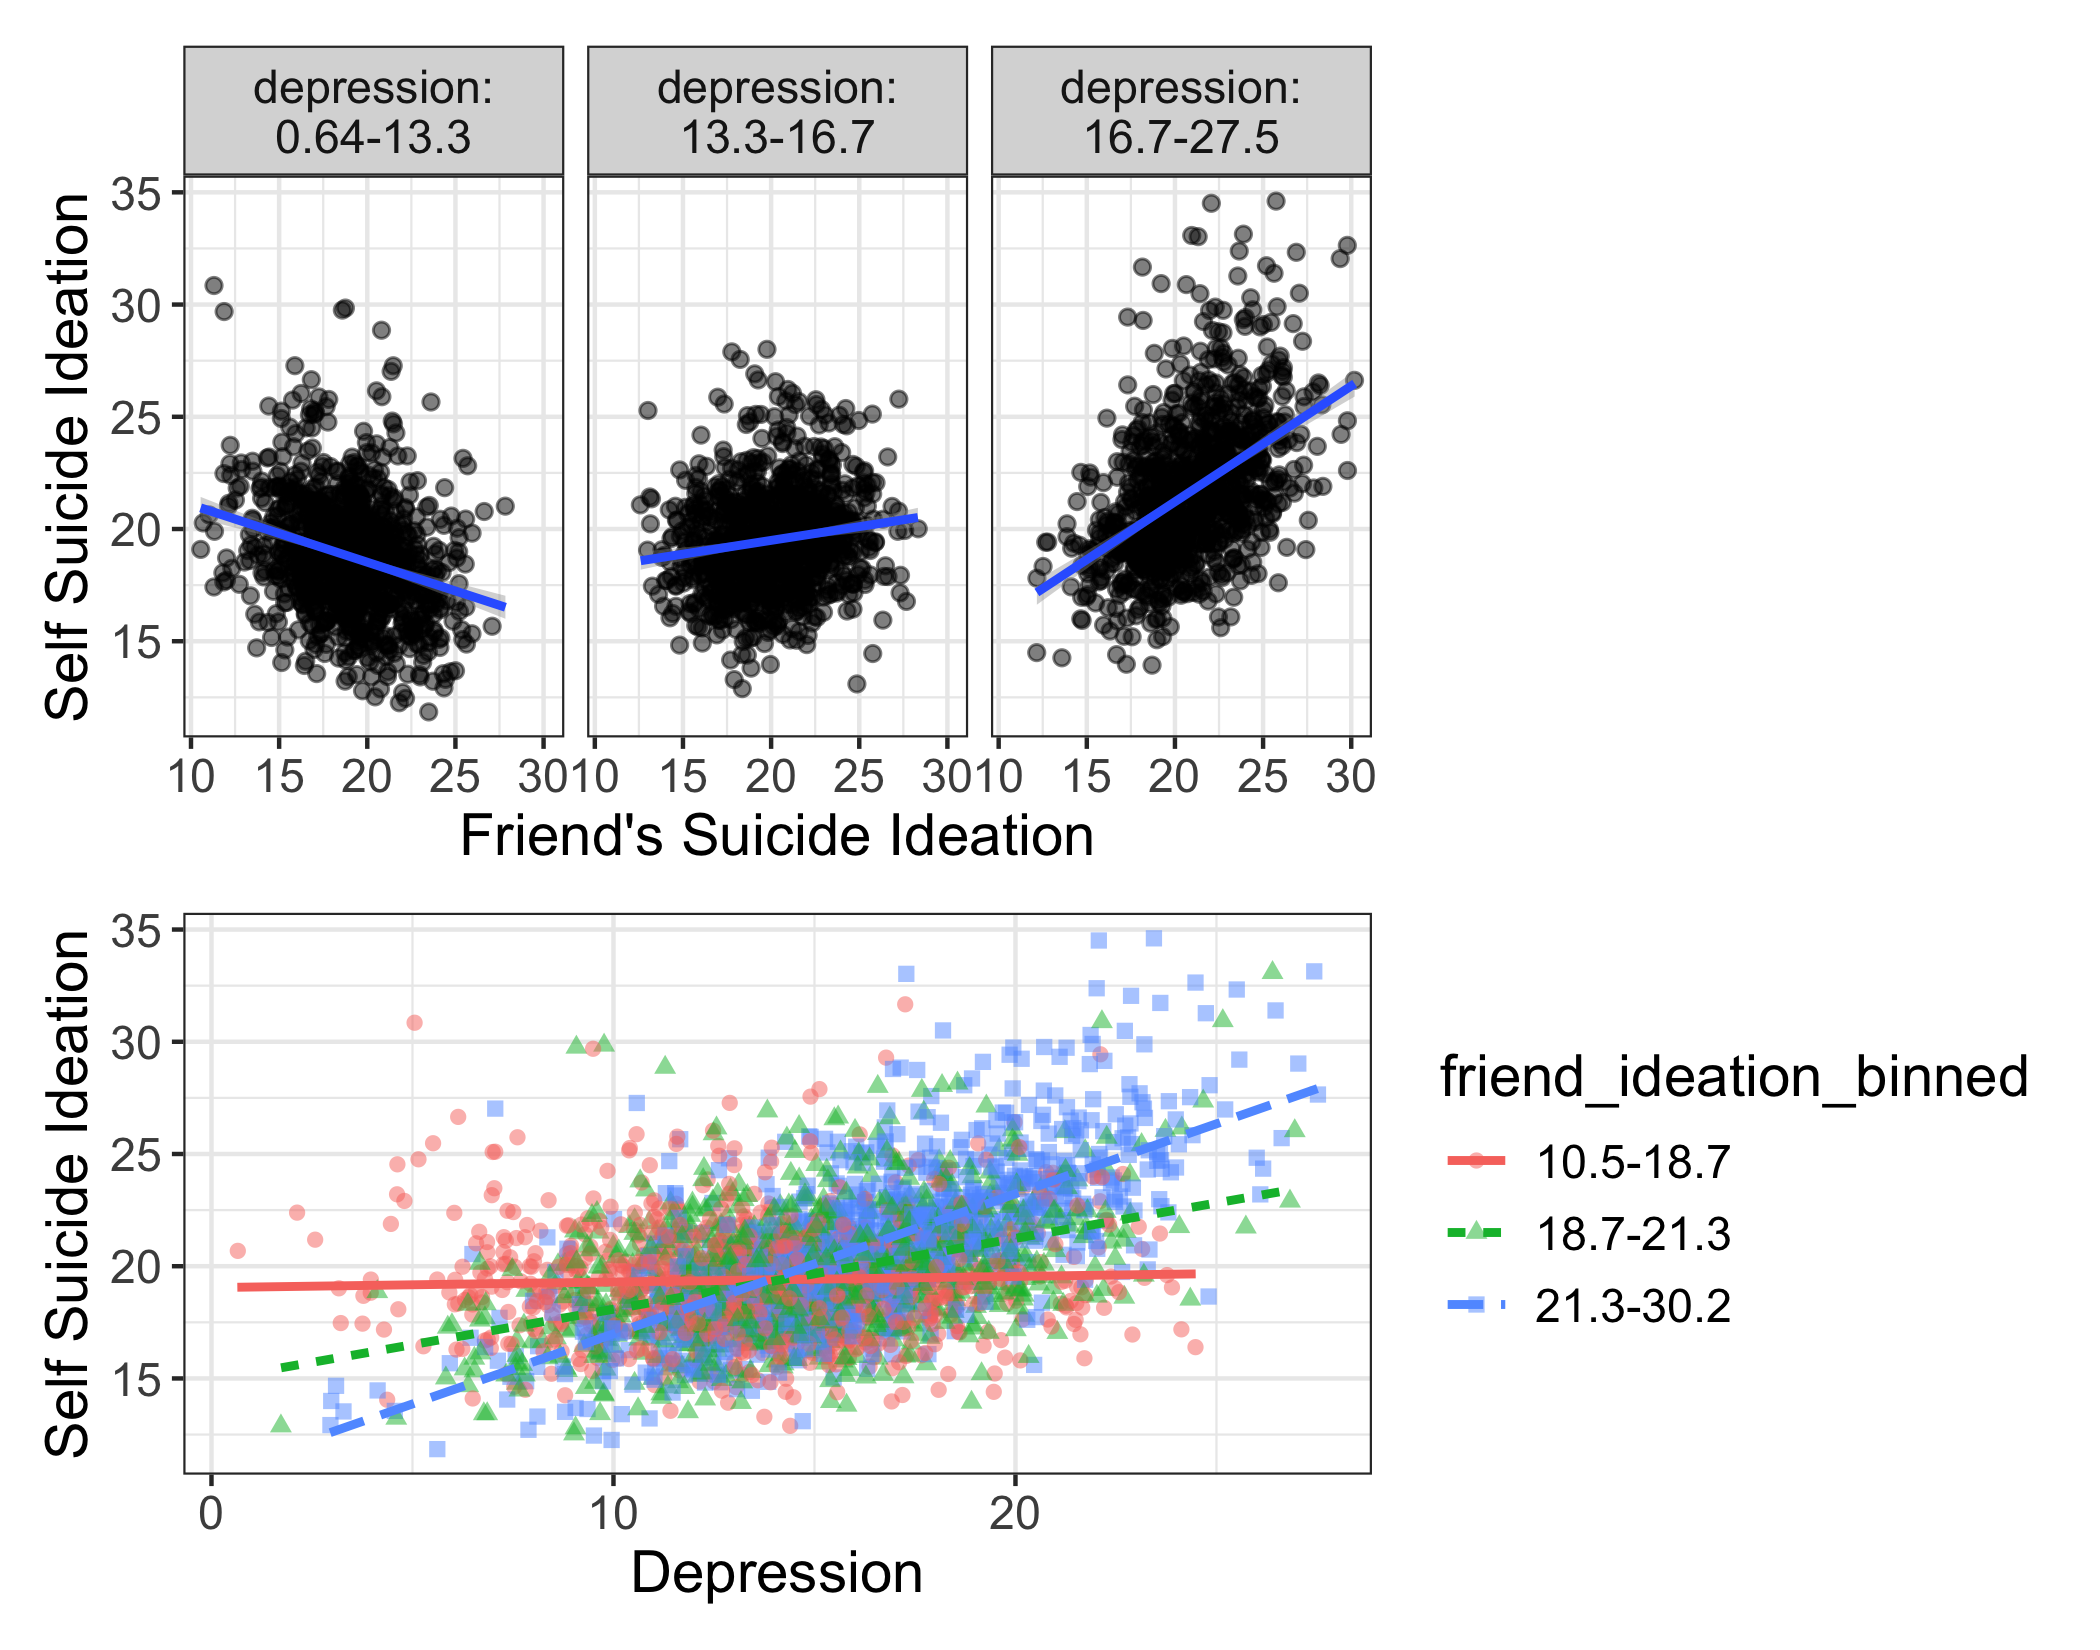
\includegraphics[width=0.7\linewidth]{visual_partitions_files/figure-latex/flexplotexample-1} 

}

\caption{These plots show examples of Flexplot graphics. In the top image,  lines/colors/symbols.}\label{fig:flexplotexample}
\end{figure}

In Flexplot, the foundation of nearly all graphics is a simple bivariate scatterplot. Technically, ``flexplot'' is the suite of tools within the flexplot package that are used for visualization. However, quite by accident and without the author's persuasions, ``flexplots'' have become somewhat synonymous with ``paneled plots.'' In those plots, additional variables are encoded using separate panels (and sometimes separate colors/symbols/lines). For example, Figure \ref{fig:flexplotexample} shows the plots for the data displayed in Table \ref{tab:anovatab}. The top image encodes a second predictor as different panels, while the lower image encodes the second predictor as separate lines/colors/symbols. In both cases, the images reveal the nature of the interaction between friend ideation and depression: depression increases suicide ideation more when one's friends also are high in suicide ideation, relative to when one's friends are low in suicide ideation.

\begin{figure}

{\centering 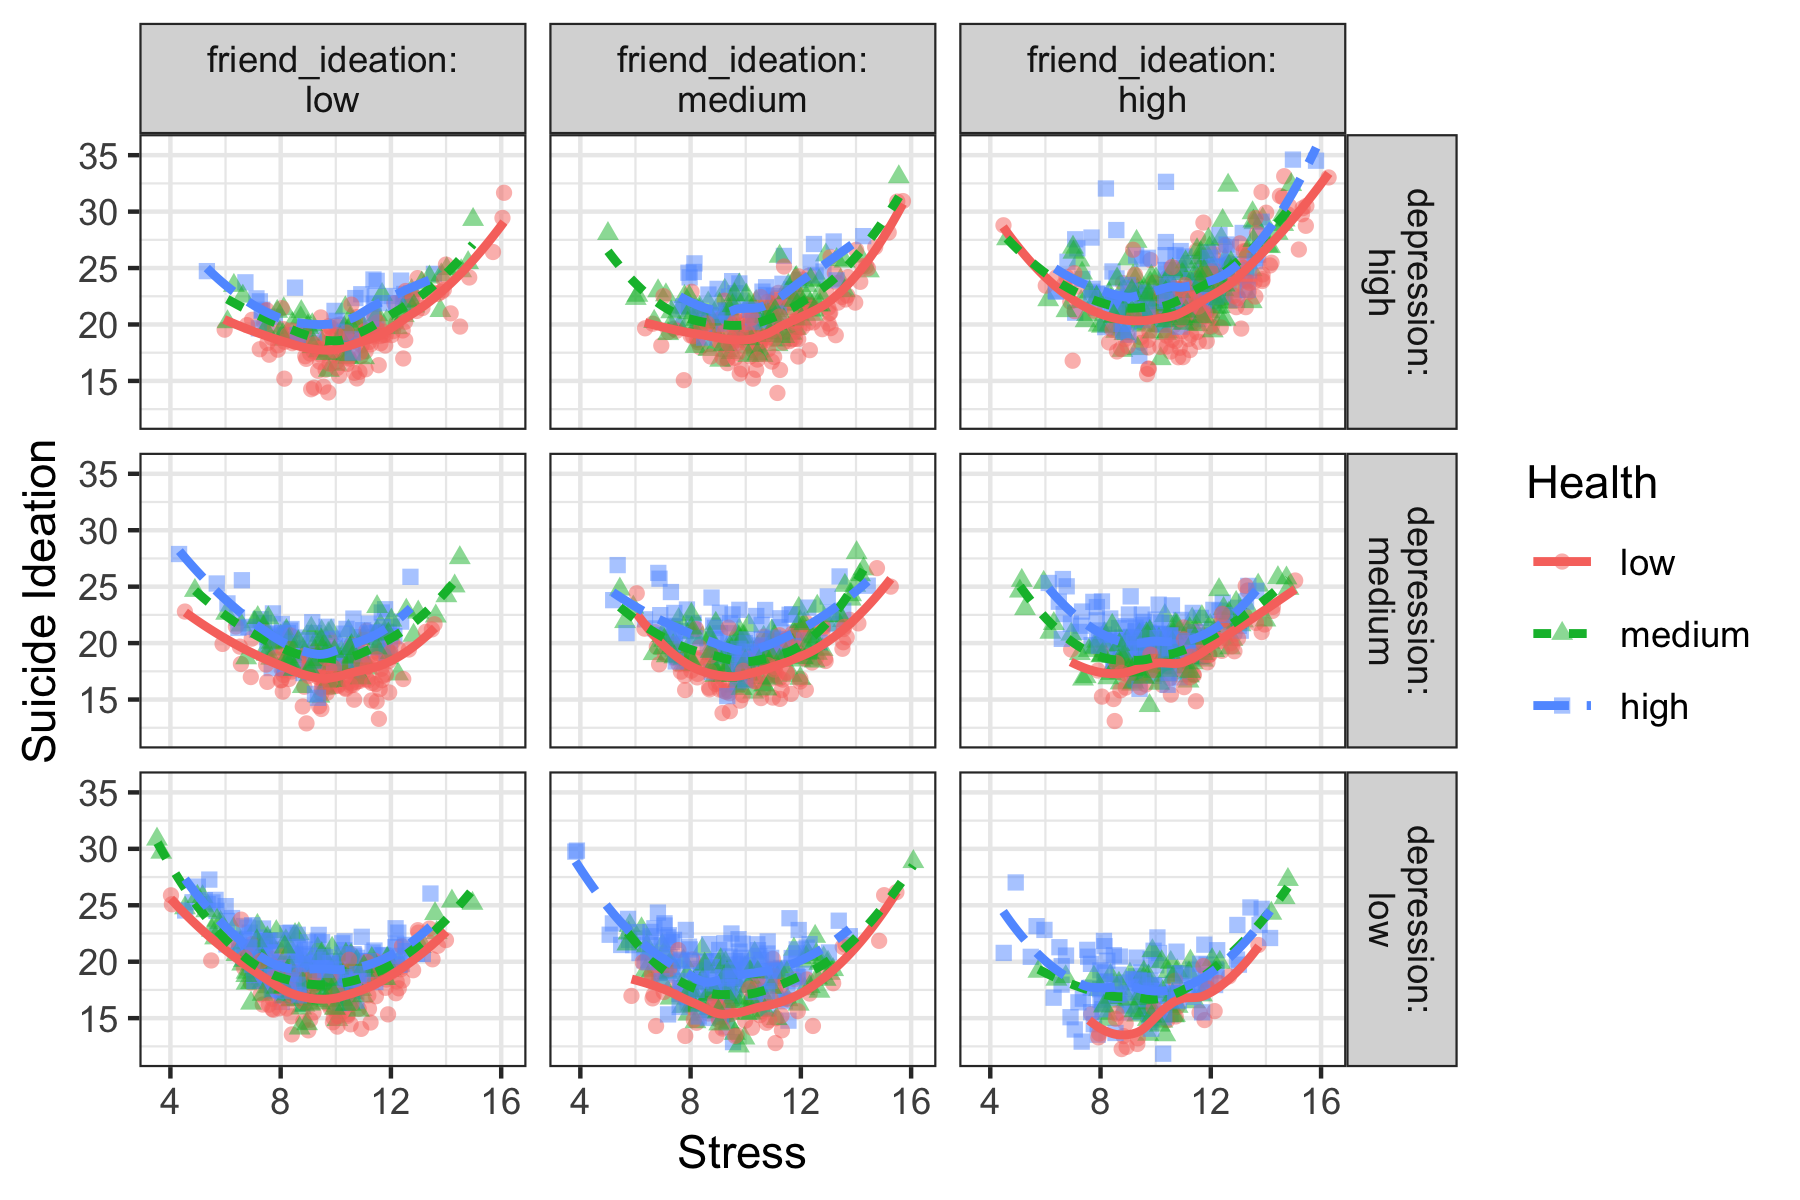
\includegraphics[width=0.75\linewidth]{visual_partitions_files/figure-latex/flexplotequation-1} 

}

\caption{This image shows the suicide ideation data with a Flexplot graphic. Stress is shown on the $X$-axis, health is separated into bins and different values are shown as colors/symbols/lines, and friend ideation/depression are also binned and displayed in separate panels.}\label{fig:flexplotequation}
\end{figure}

When using Flexplot in R, relationships can be specified in R using a Flexplot equation of the following form: \texttt{y\ \textasciitilde{}\ a\ +\ b\ \textbar{}\ c\ +\ d}. The variable \texttt{y} is displayed on the \(Y\)-axis, \texttt{a} is on the \(X\)-axis, \texttt{b} is displayed as separate colors/symbols/lines, \texttt{c} is shown in row panels, and \texttt{d} is shown in column panels. As an example, consider Figure \ref{fig:flexplotequation}, which plots the relationship between stress/depression/friend ideation and suicide ideation. The command used to generate these data was \texttt{flexplot(ideation\textasciitilde{}stress\ +\ health\ \textbar{}\ friend\_ideation\ +\ depression,\ data=ideation)}.

Flexplot defaults to overlaying ``loess'' lines (Cleveland, 1993), which are nonparametric smoothing functions that can bend with the data. The reason for this default is that loess lines will reveal any nonlinear relationships between the predictor and outcome variable. For example, Figure \ref{fig:flexplotequation} reveals the nonlinear relationship between suicide ideation and stress: initially, increasing stress reduces ideation, but after around stress scores of 10, increasing stress increases suicide ideation.

Flexplot also makes it easy to identify interaction effects; interactions will show up as nonparallel lines across either panels or colors/lines/symbols. However, with so many panels it is easy to experience information overload and fail to identify patterns of nonparallel lines. The next tool, however, makes it easy to identify nonparallel lines in a Flexplot graphic.

\subsection{Tool \#2: Marginal Plots}\label{tool-2-marginal-plots}

The second tool I will utilize is what I call a ``marginal plot.'' These too are available in the R package \texttt{flexplot} (as of version 0.10).\footnote{Marginal plots are different than ``marginal-effects plots'' (Berry, Golder, \& Milton, 2012; Preacher, Curran, \& Bauer, 2006), which plot the slope of \(X\) against a moderator (e.g., \(Z\)).} Marginal plots make it easy to detect interactions.

\begin{figure}

{\centering 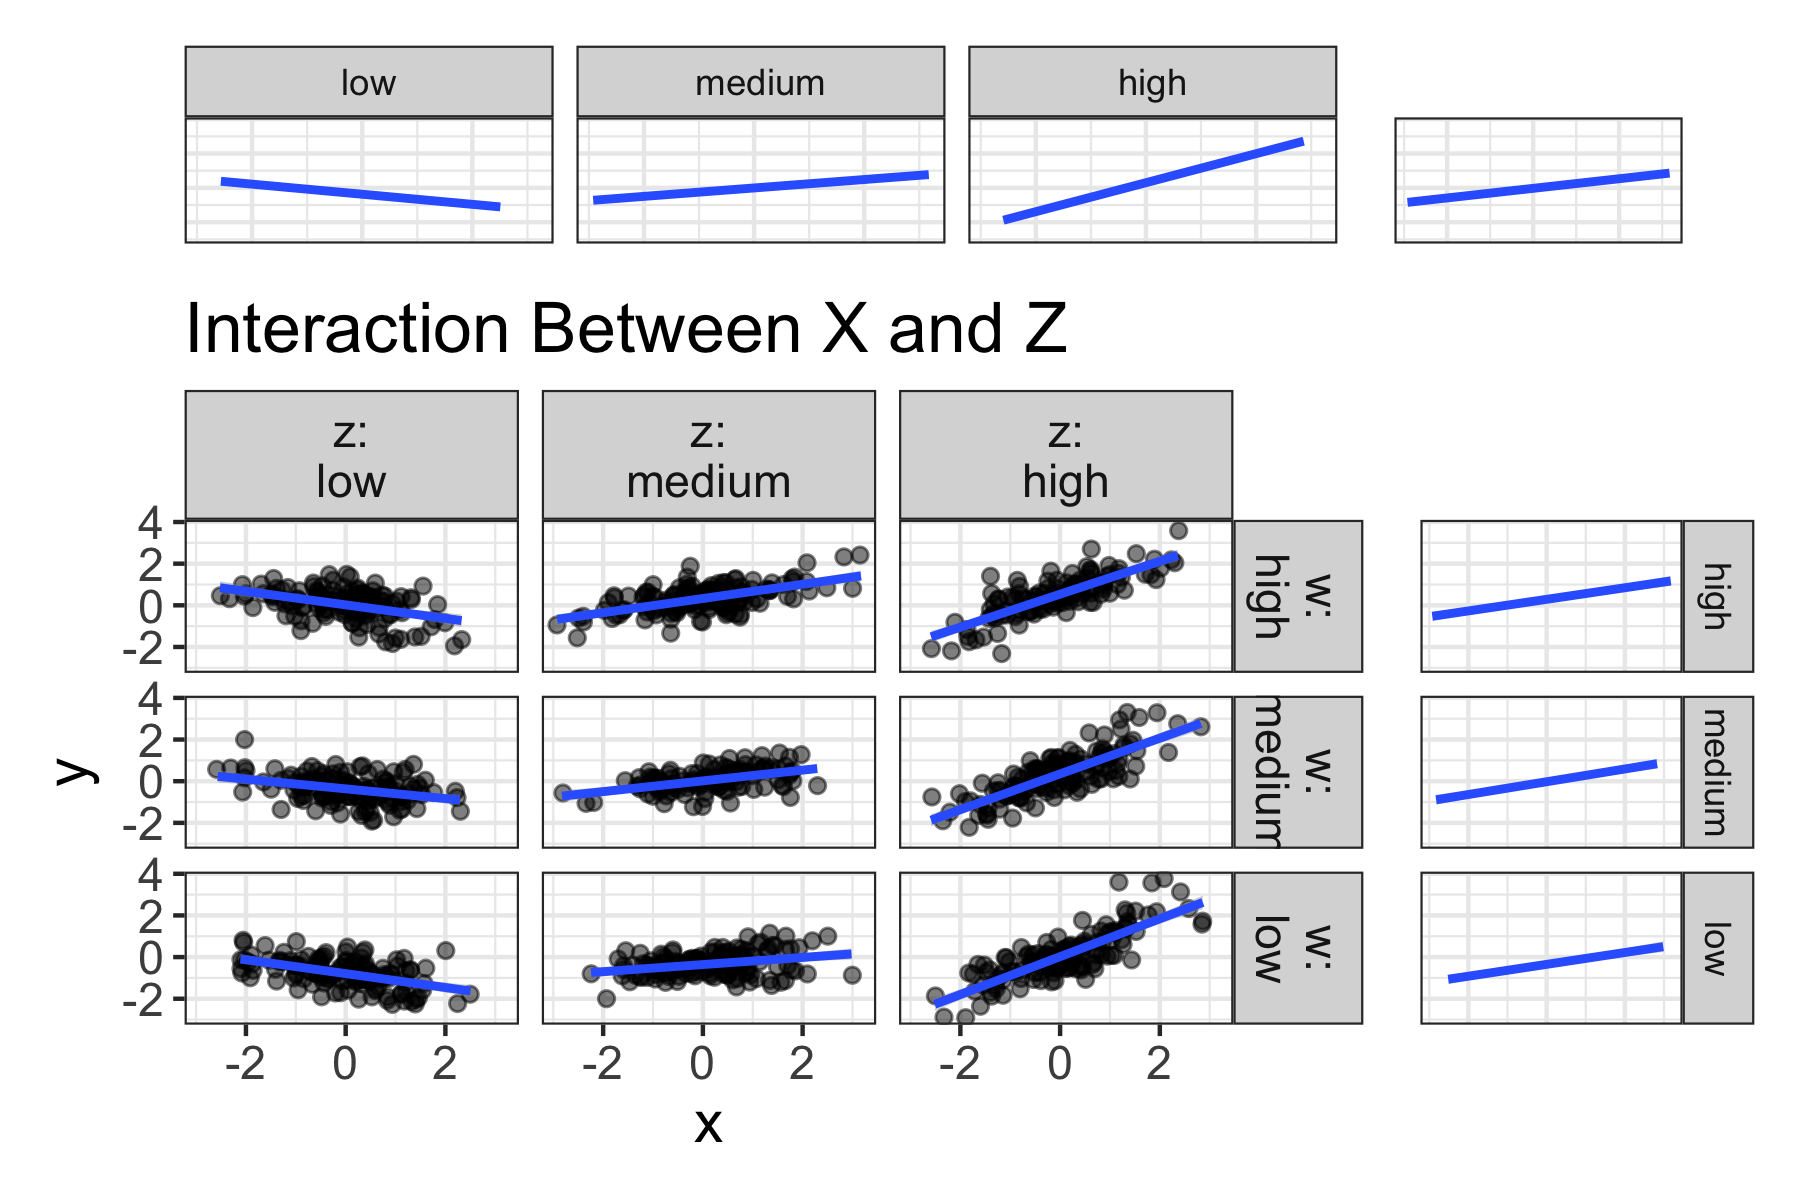
\includegraphics[width=0.75\linewidth]{visual_partitions_files/figure-latex/threeinteractions1-1} 

}

\caption{This shows an example of a marginal plot where $X$ interacts with $Z$ only. The marginal plot shows non-parallel slopes across the columns.}\label{fig:threeinteractions1}
\end{figure}

Recall that Flexplot allows one to plot multivariate relationships (as in Figure \ref{fig:flexplotequation}). These plots can be used to detect interactions by identifying whether the slopes are parallel across each of the panels (or across the different lines/colors/symbols). If the lines are not parallel, one of the variables (either the variable in the row panel, the variable in the column panel, or the variable represented as a color/line/symbol) interacts with the variable on the \(X\)-axis. More specifically,

\begin{itemize}
\tightlist
\item
  if lines systematically deviate from parallel as a function of the columns, the variable on the \(X\)-axis interacts with the variable in column panels
\item
  if lines systematically deviate from parallel as a function of the rows, the variable on the \(X\)-axis interacts with the variable in row panels
\item
  if lines systematically deviate from parallel as a function of the colors/lines/symbols, the variable on the \(X\)-axis interacts with the variable represented as a color/line/symbol
\item
  if lines systematically deviate from parallel as a function of rows and/or colors and/or columns, there's possibly a three or four-way interaction
\end{itemize}

While the rules are simple, it becomes difficult to visually aggregate across panels (or colors/lines/symbols) using Flexplot alone. To assist with this visual aggregation, marginal plots produce three additional groups of plots: the plots above the Flexplot will show the average slope for each column panel, aggregated across the row panels. The plots to the right of the Flexplot will show the average slope for each row panel, aggregated across the column panels. The top-right plot will show the average slope for \(X\), averaged across both rows and columns. (Unfortunately, marginal plots do not average across colors/symbols/lines).

\begin{figure}

{\centering 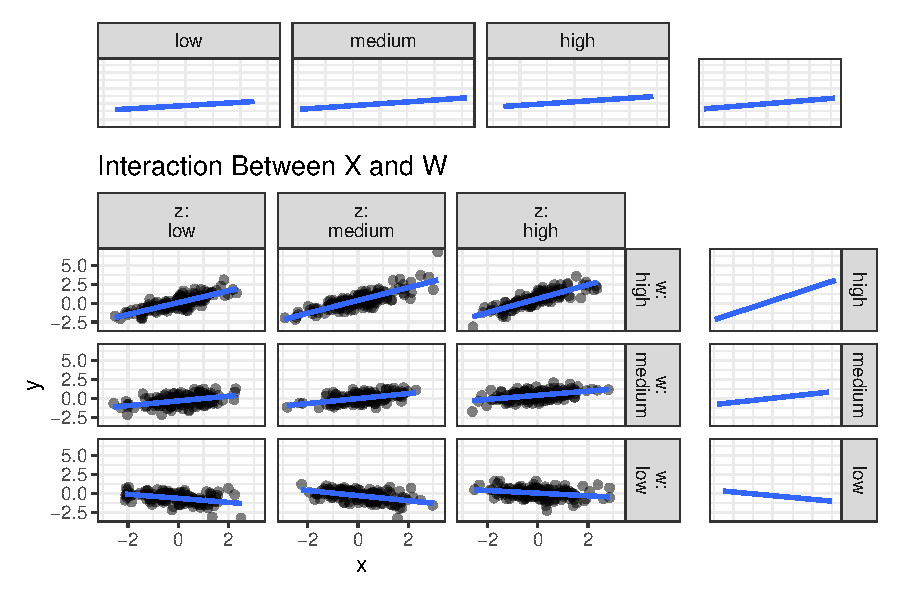
\includegraphics[width=0.75\linewidth]{visual_partitions_files/figure-latex/threeinteractions2-1} 

}

\caption{Example of a marginal plot where $X$ interacts with $W$ only. The marginal plot shows non-parallel slopes across the rows.}\label{fig:threeinteractions2}
\end{figure}

Figures \ref{fig:threeinteractions1}-\ref{fig:threeinteractions3} shows examples of several of these conditions. The first plot (Figure \ref{fig:threeinteractions1}) shows an interaction between \(X\) and the variable in the column panels (\(Z\)). Notice that the row plots seem to be fairly parallel, while the column plots increase their slope as \(Z\) increases. The second plot (Figure \ref{fig:threeinteractions2}) shows an interaction between \(X\) and the variable in the row panels (\(W\)). Now, the column plots are fairly parallel, while the row plots go from negative to positive. Finally, (Figure \ref{fig:threeinteractions3}) shows a three-way interaction. Here, the marginal plots suggest the rows and columns are parallel. However, notice that, within the 9-panel grid of the raw data, the slopes are \emph{not} parallel. For these particular data, the data were simulated to have a three-way interaction, but no two-way interactions. Alternatively, both the row and the column margins might be nonparallel, which might indicate the variables have both two-way and three-way interactions present.

\begin{figure}

{\centering 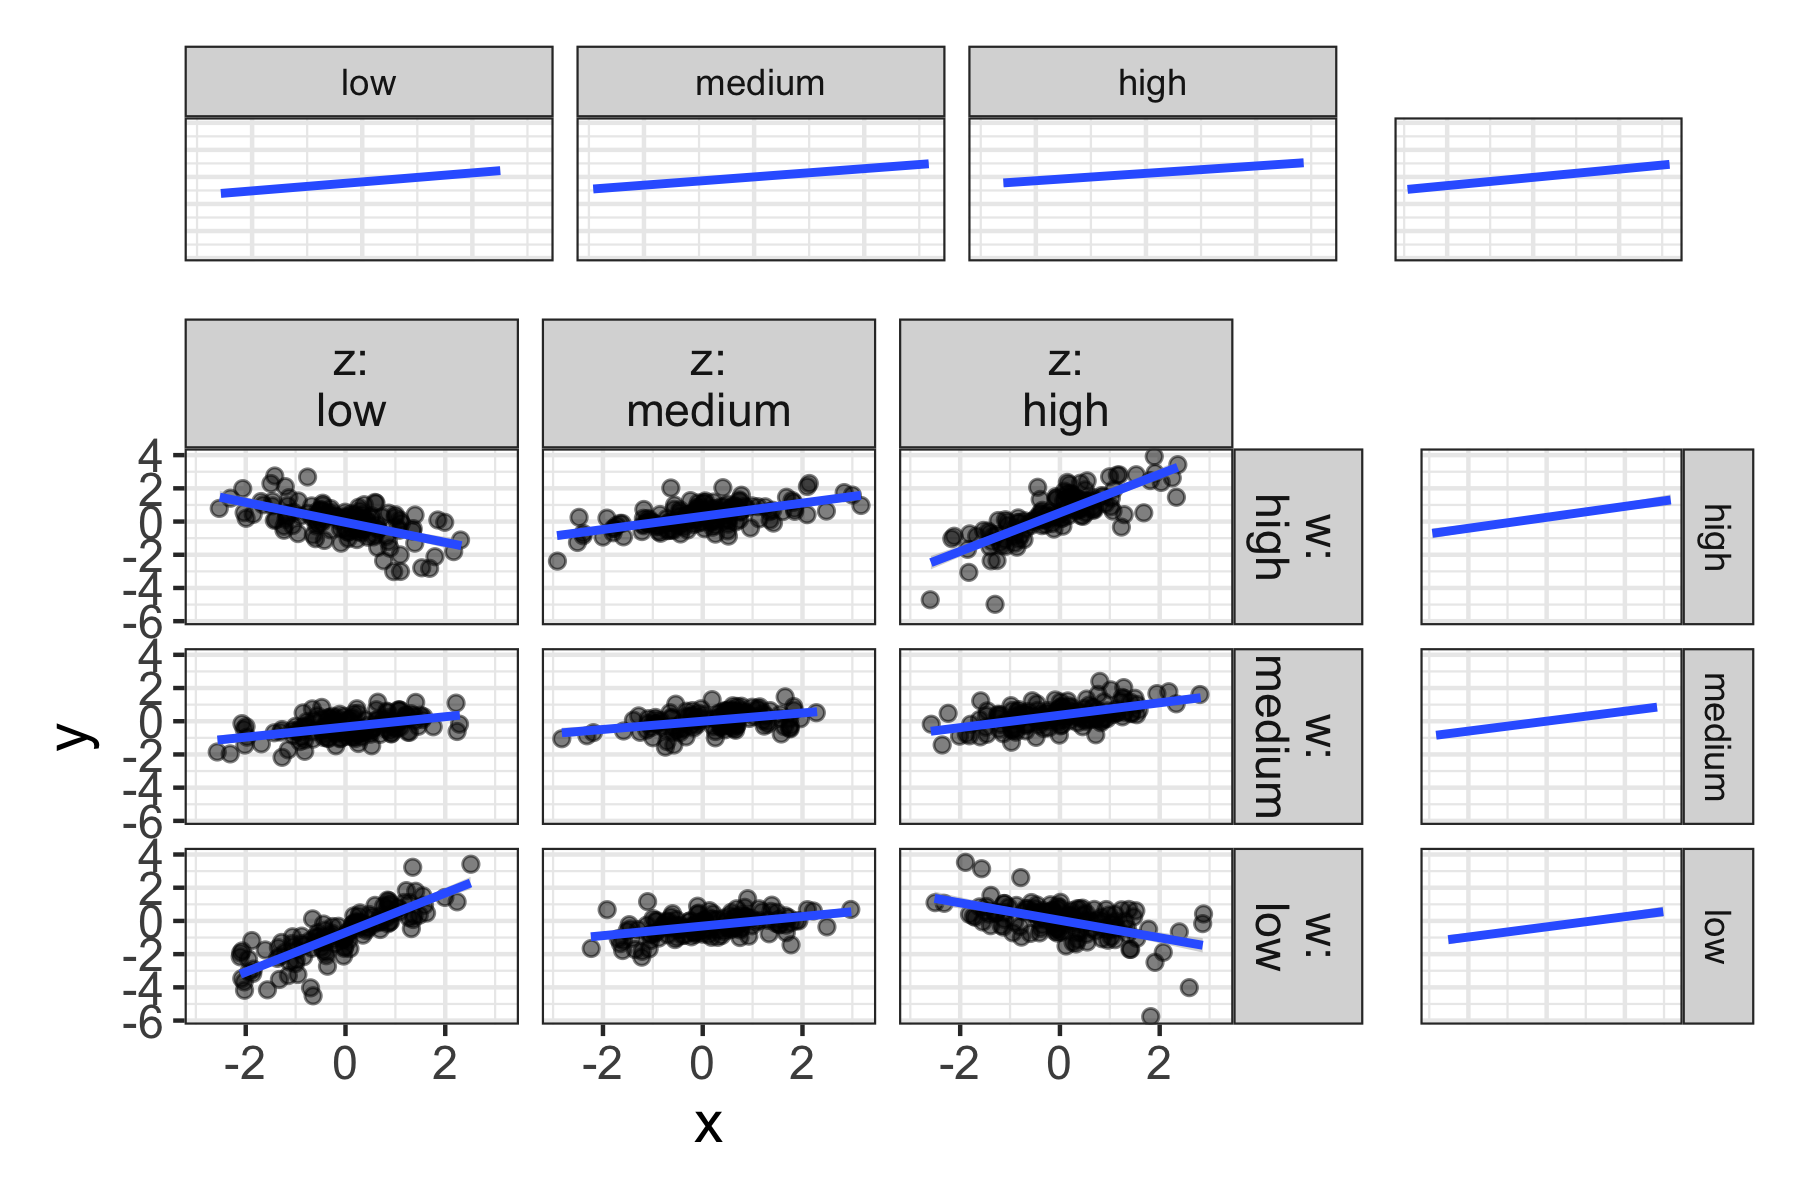
\includegraphics[width=0.75\linewidth]{visual_partitions_files/figure-latex/threeinteractions3-1} 

}

\caption{Example of a marginal plot where $X$ interacts with $W$ and $Z$. The marginal plot shows parallel slopes across the rows and panels, but the raw data in the 9x9 grid show nonparallel lines.}\label{fig:threeinteractions3}
\end{figure}

In short, marginal plots are a valuable tool in identifying whether variables interaction, as well as identifying \emph{how} they interact.

\subsection{Tool \#3: Partial Residual Plots}\label{tool-3-partial-residual-plots}

Partial residual plots (Ezekiel, 1924; Larsen \& McCleary, 1972) are another useful (though rarely used) tool for data analysis. The goal of partial residual plots (PRPs) is to visualize the conditional effect of a variable (i.e., the effect of a predictor variable, after controlling for another predictor or multiple predictors). For simplicity, I will call the variable we wish to control the ``covariate'' and the variable for which we wish to determine the effect the ``interest variable.''

Suppose we have a statistical model of the form \(y = b_0 + b_1 X + b_2 Z\). Further suppose we consider \(X\) to be our covariate and \(Z\) to be our interest variable. We know that the parameter associated with \(Z\) (\(b_2\)) is to be interpreted as the slope of \(Z\), \emph{after controlling for the effects of \(X\)}, or \emph{holding \(X\) constant.} How does one visualize this effect?

PRPs are one approach for visualizing the net effect of one variable, conditional on another. PRPs were invented by Ezekiel (1924), then independently reinvented by Larsen and McCleary (1972). Plotting a PRP is a four-step process:

\begin{enumerate}
\def\labelenumi{\arabic{enumi}.}
\tightlist
\item
  Fit the entire statistical model (for example, \(y = b_0 + b_1 X + b_2 Z\)).
\item
  Calculate the residuals from Step \#1. We will call these residuals \(e_{Y|X + Z}\).
\item
  Calculate the residuals with only the \(X\) effect removed (but not the \(Z\) effect). We will call these residuals \(e_{Y|X \neg Z}\). To calculate these, we add the fitted values for \(Z\) back to the residuals: \(e_{Y|X \neg Z} = e_{Y|X + Z} + \beta_Z \times Z\).
\item
  Plot the \(Z\) variable against these new residuals (\(e_{Y|X \neg Z}\)).
\end{enumerate}

Let us carefully consider what these plots are telling us. Recall that residuals tell us the portion of the outcome the model failed to fit. In this case, the residuals tell us what parts of \(y\) could not be fit with either \(X\) or \(Z\). When we then add back in the fit of \(X\) (Step 3), the residuals tell us what neither \(X\) nor \(Z\) were able to fit \emph{plus} the part that \(X\) \emph{was} able to fit. Put differently, these new residuals control for the effect of \(Z\), but not \(X\). When we then plot the raw \(X\) values against these new residuals, the resulting plot will yield an accurate representation of the \emph{unique} effect of \(X\) on the outcome. Furthermore, the slope of the plotted line is \emph{exactly} equal to \(b_2\).\footnote{An alternative to PRPs is an added variable plot (Kutner, Nachtsheim, Neter, \& Li, 2004). The idea behind added variable plots (AVPs) is very similar to PRPs; they are designed to visualize a conditionalized effect. With AVPs, we fit a model between the covariate (e.g., \(Z\)) and the outcome (e.g., \(Y\)), extract the residuals, then plot these residuals against the interest variable (e.g., \(X\)). AVPs then are a visual approximation of the model where X and Z are predictors of Y. However, because the interest variable isn't actually modeled, it is only an approximation and the slope in the AVP is not identical to the slope from the multivariate model, as they are in the PRP.} As such, these are a precise visual representation of the statistical model.

PRPs are enormously helpful for visualizing multivariate relationships simply because they convert a complex multivariate relationship (e.g., the model \(y = b_0 + b_1 X + b_2 Z\)) into simple bivariate scatterplots. In this case, we could have a PRP for the \(X\) effect and one for the \(Z\) effect. However, this simplification is \emph{only} merited if the statistical model doesn't contain unmodeled interactions or nonlinear terms. If there are unmodeled multiplicative (interaction or nonlinear) effects, the simple main effects are biased and misleading. Granted, one could model these multiplicative effects and the statistical estimates will be unbiased. However, multiplicative effects render the ``main effects'' (or marginal effects) uninterpretable (Appelbaum \& Cramer, 1974); variables with multiplicative effects must be interpreted in the context of the other variable(s) involved in the multiplicative effect. For example, suppose we're interested in studying the effects of rot on degree of food poisoning. If our sample consists of both vultures and humans, we're going to have a very strong interaction effect: for vultures, there's no relationship between rot and food poisoning, while for humans there is a very strong effect. In this case, it make no sense to discuss the main effect of rot on food poisoning because \emph{it depends} on species, and any interpretation of these variables in isolation is misleading. Likewise, a traditional bivariate PRP will be misleading if there are multiplicative effects. This seriously limits the usefulness of traditional PRPs since multiplicative effects are quite common (Cronbach, 1975). Fortunately, the traditional PRP can be slightly modified to accommodate situations where multiplicative effects are present. In the next section, I introduce a multivariate extension of the PRPs that will accomplish this goal.

\subsubsection{Multivariate Extensions of PRPs}\label{multivariate-extensions-of-prps}

The multivariate extension of the PRP follows the same procedure as the original approach. Now, however, the user can specify more complex statistical models in Step \#1 (e.g., \(y = b_0 + b_1 X + b_2 Z +b_3 X^2 + b_4 X\times Z\)). Also, one can take a flexplot approach and visualize multiple variables simultaneously (e.g., plot \(X\) on the \(X\)-axis, \(W\) in panels, and the residuals on the \(Y\)-axis). Now, however, one would add back in the residuals of multiple variables (e.g., \(X\) \emph{and} \(W\)) in Step \#3.

This can all be done in the Flexplot package in R (as of version 10.0.2.1), using the function \texttt{partial\_residual\_plot}. To do so, the function requires four arguments:

\begin{enumerate}
\def\labelenumi{\arabic{enumi}.}
\tightlist
\item
  \textbf{A Flexplot equation that specifies how variables are to be plotted.} As before, we use an equation of the form \texttt{y\textasciitilde{}a+b\textbar{}c+d}, or any of its variations (e.g., \texttt{y\textasciitilde{}a\textbar{}b}, which places \(b\) in panels, or \texttt{y\textasciitilde{}a+b}, which plots different lines/colors/symbols for different levels of \(b\)).
\item
  \textbf{The multivariate model.} This model may contain any number of predictors, nonlinear terms, and/or interaction components. As of this writing, the \texttt{partial\_residual\_plot} function requires the model to be an \texttt{lm} model, though future versions of Flexplot will extend this functionality to additional models (e.g., \texttt{glm}, or \texttt{rlm} models).
\item
  \textbf{Which terms in \#2 are going to be added back to the residuals from the model.} Note that the terms added back must involve the same variables used in Step 1 (e.g., if one specifies \texttt{y\textasciitilde{}a\textbar{}b} in Step 1, the terms added back might be \texttt{a\ +\ a\^{}2\ +\ b\ +\ a:b}, each of which involves the variables \texttt{a} and \texttt{b}.)
\item
  \textbf{The dataset}
\end{enumerate}

\begin{figure}

{\centering 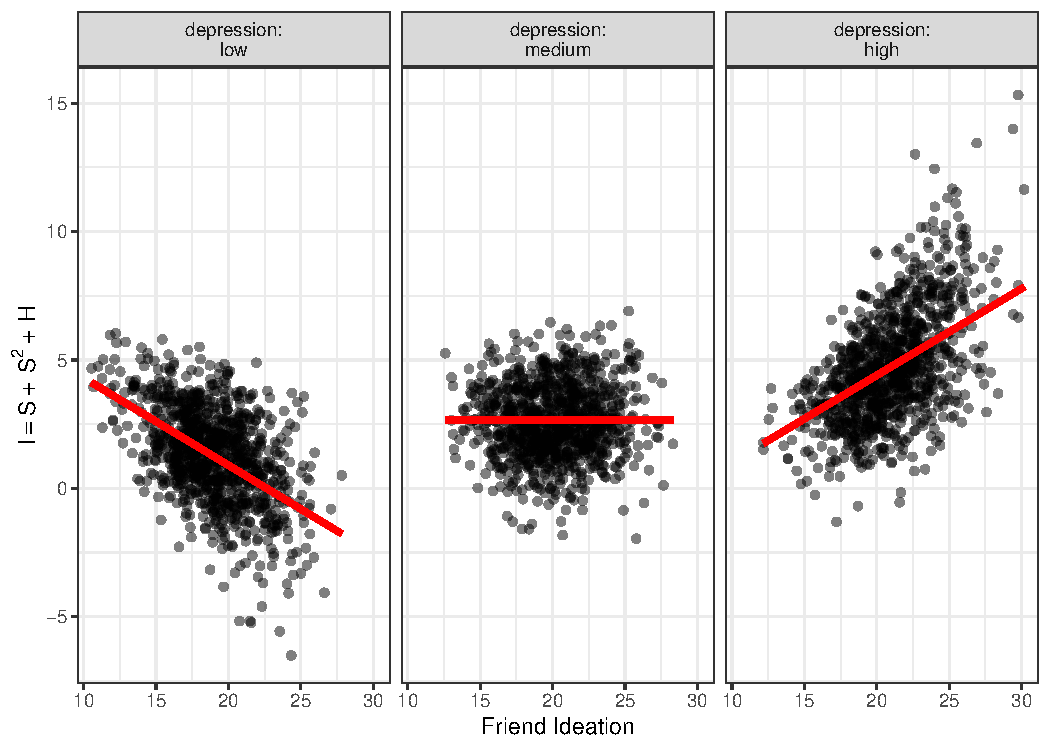
\includegraphics[width=0.7\linewidth]{visual_partitions_files/figure-latex/prp1a-1} 

}

\caption{This plot shows a multivariate partial residual plot of the friend ideation/depression relationship, conditional on stress and health. I = ideation, S = Stress, H = Health.}\label{fig:prp1a}
\end{figure}

The code below demonstrates how to do this in R. This code first fits the entire model from Equation \eqref{eq:model} (where ideation is predicted from health, stress, a quadratic stress term, depression, friend ideation, and the interaction between friend ideation and depression). Subsequently, we use the \texttt{partial\_residual\_plot} function to specify the Flexplot equation for graphing (\texttt{ideation\textasciitilde{}friend\_ideation\textbar{}depression}), which will plot friend\_ideation on the \(X\)-axis and depression in panels. We also specify the \texttt{added\_term} argument, which specifies which terms to add back into the residuals (in this case \texttt{\textasciitilde{}depression*friend\_ideation}, which will add back to the residuals the main effects and interactions from depression and friend\_ideation). Additional arguments are added for visual clarity (including labeling the axes). The resulting plot is shown in Figure \ref{fig:prp1a}

\begin{Shaded}
\begin{Highlighting}[]
\FunctionTok{require}\NormalTok{(flexplot)}
\CommentTok{\# fit the multivariate model}
\NormalTok{model }\OtherTok{=} \FunctionTok{lm}\NormalTok{(ideation}\SpecialCharTok{\textasciitilde{}}\NormalTok{stress}\SpecialCharTok{+}\FunctionTok{I}\NormalTok{(stress}\SpecialCharTok{\^{}}\DecValTok{2}\NormalTok{)}\SpecialCharTok{+} 
\NormalTok{             depression}\SpecialCharTok{*}\NormalTok{friend\_ideation }\SpecialCharTok{+} 
\NormalTok{             health, }
           \AttributeTok{data=}\NormalTok{ideation)}
\CommentTok{\# plot the PRP}
\FunctionTok{partial\_residual\_plot}\NormalTok{(ideation}\SpecialCharTok{\textasciitilde{}}\NormalTok{friend\_ideation }\SpecialCharTok{|}\NormalTok{ depression, }
                      \AttributeTok{model=}\NormalTok{model, }
                      \AttributeTok{added\_term =} \SpecialCharTok{\textasciitilde{}}\NormalTok{depression}\SpecialCharTok{*}\NormalTok{friend\_ideation, }
                      \AttributeTok{data=}\NormalTok{ideation) }\SpecialCharTok{+}
  \CommentTok{\# modify the labels}
  \FunctionTok{ylab}\NormalTok{(}\FunctionTok{expression}\NormalTok{(I}\SpecialCharTok{==}\NormalTok{S}\SpecialCharTok{\textasciitilde{}+}\ErrorTok{\textasciitilde{}}\NormalTok{S}\SpecialCharTok{\^{}}\NormalTok{\{}\DecValTok{2}\NormalTok{\}}\SpecialCharTok{\textasciitilde{}+}\ErrorTok{\textasciitilde{}}\NormalTok{H)) }\SpecialCharTok{+} 
  \FunctionTok{xlab}\NormalTok{(}\StringTok{"Friend Ideation"}\NormalTok{) }\SpecialCharTok{+}
  \FunctionTok{theme\_bw}\NormalTok{()}
\end{Highlighting}
\end{Shaded}

Now, suppose we wished to visualize the stress effect. The stress effect does not interact with other variables but it does have a nonlinear relationship with the outcome. As before, we might pass the fitted multivariate model to the \texttt{partial\_residual\_plot} function as before, but our Flexplot formula would be \texttt{ideation\textasciitilde{}stress}. We also tell the function to add the terms \texttt{\textasciitilde{}stress} and \texttt{I(stress\^{}2)} back to the residuals of the model so we can visualize the totality of the stress effect. The code below produces the plot in Figure \ref{fig:prp2}:

\begin{Shaded}
\begin{Highlighting}[]
\CommentTok{\# plot stress on the x{-}axis, and remove it\textquotesingle{}s linear and nonlinear components}
\FunctionTok{partial\_residual\_plot}\NormalTok{(ideation}\SpecialCharTok{\textasciitilde{}}\NormalTok{stress, }
                      \AttributeTok{model=}\NormalTok{model, }
                      \AttributeTok{added\_term =} \SpecialCharTok{\textasciitilde{}}\NormalTok{stress }\SpecialCharTok{+} \FunctionTok{I}\NormalTok{(stress}\SpecialCharTok{\^{}}\DecValTok{2}\NormalTok{), }
                      \AttributeTok{data=}\NormalTok{ideation) }\SpecialCharTok{+}
  \CommentTok{\# modify the labels}
  \FunctionTok{ylab}\NormalTok{(}\FunctionTok{expression}\NormalTok{(I}\SpecialCharTok{==}\NormalTok{H}\SpecialCharTok{\textasciitilde{}+}\ErrorTok{\textasciitilde{}}\NormalTok{D}\SpecialCharTok{\textasciitilde{}+}\ErrorTok{\textasciitilde{}}\NormalTok{FI}\SpecialCharTok{\textasciitilde{}+}\ErrorTok{\textasciitilde{}}\NormalTok{\{D\}}\SpecialCharTok{\%*\%}\NormalTok{\{FI\})) }\SpecialCharTok{+} 
  \FunctionTok{xlab}\NormalTok{(}\StringTok{"Stress"}\NormalTok{) }\SpecialCharTok{+}
  \FunctionTok{theme\_bw}\NormalTok{()}
\end{Highlighting}
\end{Shaded}

\begin{figure}

{\centering 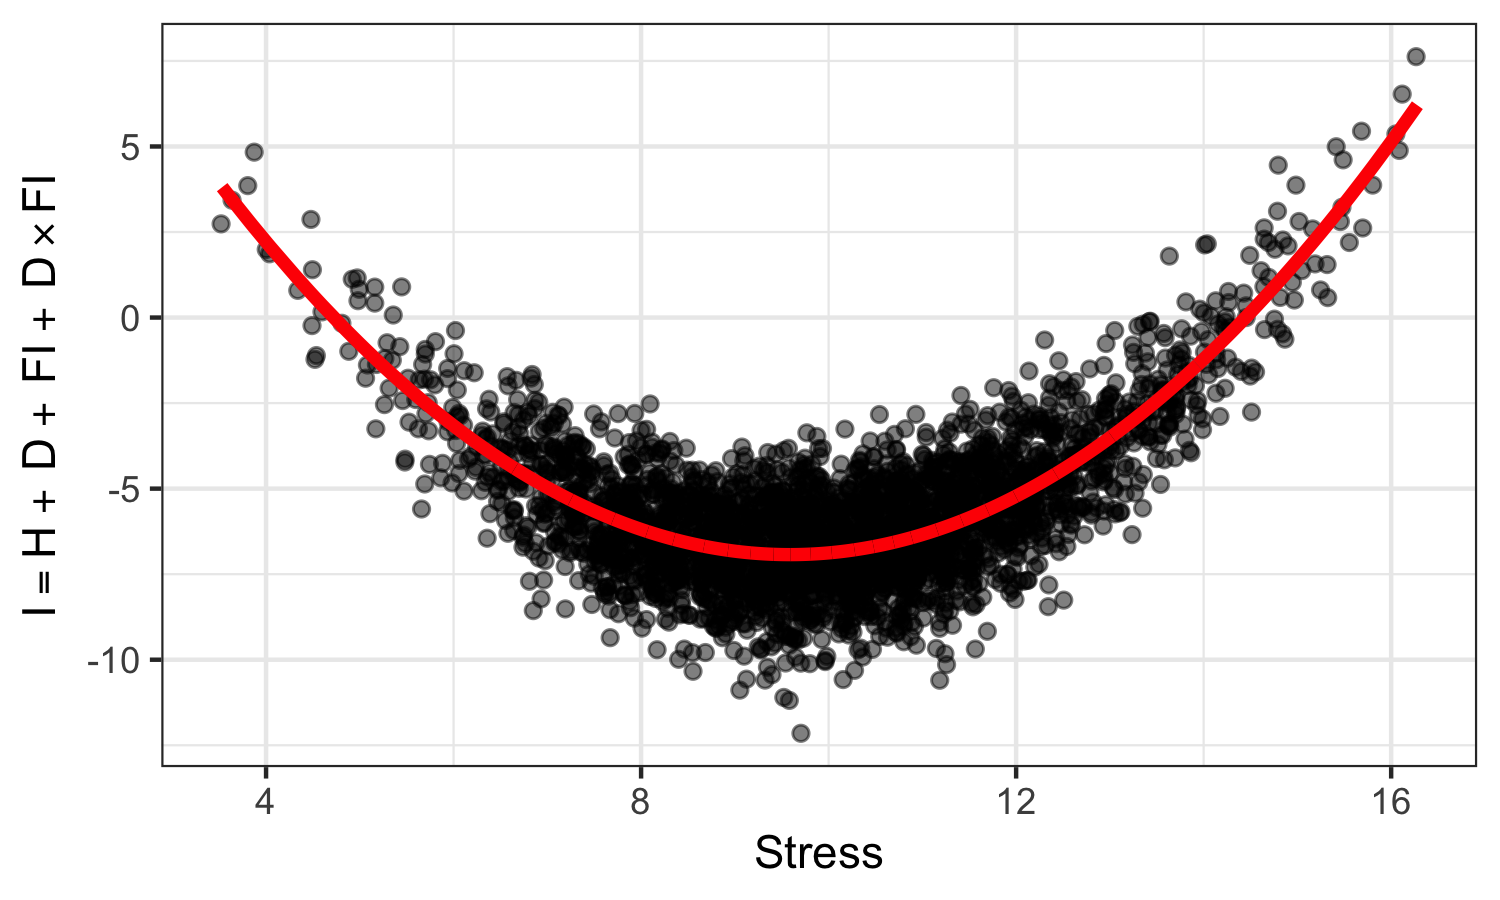
\includegraphics[width=0.75\linewidth]{visual_partitions_files/figure-latex/prp2-1} 

}

\caption{This plot shows a multivariate partial residual plot of the stress relationship, conditional on health, depression, and friend ideation. In this PRP, we add back the linear and nonlinear effects of stress. I = ideation, S = Stress, H = Health, D = Depression, FI = Friend Ideation.}\label{fig:prp2}
\end{figure}

\subsubsection{Residual Analysis with PRPs}\label{residual-analysis-with-prps}

This multivariate extension of PRPs is useful, not only because it is able to accurately visualize the conditional statistical effects, but it's also useful for identifying \emph{unmodeled} effects. To do so, one could leave the \texttt{added\_term} argument blank, which will tell the \texttt{partial\_residual\_plot} function to simply plot the residuals (instead of adding back an effect to the residuals). In this situation, these plots are similar (if not identical) to residual dependence plots\footnote{Residual dependence plots show the fitted values on the \(X\)-axis and the residuals of the model on the \(Y\)-axis. They are frequently used in model diagnostics to see whether there are unmodeled relationships between the fit of the model and the residuals (e.g., if there's nonlinearity that wasn't modeled). If one produces a bivariate graphic with a PRP without specifying any values in the \texttt{added\_term} argument, PRPs are exactly equal to the residual dependence plot. However, PRPs can also plot multivariate plots, or (as we said previously) add back fitted elements into the plot. As such, residual dependence plots are a ``special case'' of PRPs.}, which are often used to identify missing nonlinear components and/or heteroscedasticity.

For example, suppose we have a model where we fit the linear component of stress, but not the nonlinear component. In this case, residualizing from the model will have removed the lienar component of stress, but not the nonlinear effect. As such, the residuals will be nonlinearly correlated with the stress effect. If we then plot stress as a PRP without adding any terms back to the model, the raw data will display a nonlinear relationship (which indicates that our model failed to capture the nonlinear effect of stress on the outcome). Figure \ref{fig:missingnonlin} shows that result. These sorts of residual analysis plots are a critical component of the visualization strategy we will soon recommend.

\begin{figure}

{\centering 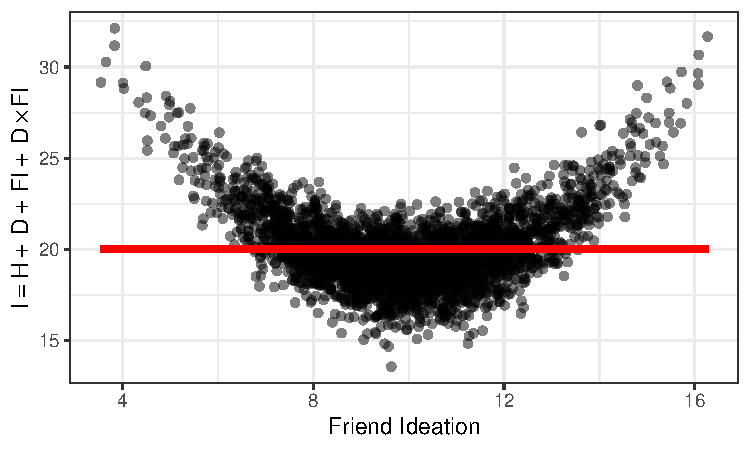
\includegraphics[width=0.75\linewidth]{visual_partitions_files/figure-latex/missingnonlin-1} 

}

\caption{This figure shows a PRP of stress against the model that includes the linear, but not the nonlinear terms of stress. In this situation, PRPs are identical to partial residual plots, which highlight sources of unmodeled nonlinearity.}\label{fig:missingnonlin}
\end{figure}

In summary, we have three tools that will serve multiple purposes as we pursue visual partitions:

\begin{enumerate}
\def\labelenumi{\arabic{enumi}.}
\tightlist
\item
  Flexplot, which enables us to visualize nonlinear effects as well as multiple variables simultaneous.
\item
  Marginal plots, which enable us to simplify a flexplot graphic and identify which variables are interacting with one another.
\item
  Partial residual plots, which allow us to visually represent conditional relationships (as well as perform residual analyses).
\end{enumerate}

In the following section, we will discuss how to obtain unbiased representations of linear models (called visual partitions), as well as identify the rules required for these visual partitions to be unbiased.

\section{Rules and Assumptions and Visual Partitions}\label{rules-and-assumptions-and-visual-partitions}

For this paper, we assume the researcher is using linear models. This class of models includes t-tests, ANOVAs, Factorial ANOVAs, ANCOVAs, and multiple regression (Cohen, 1968). With minor modifications, our visual modeling approach can be extended to additional model types, including mixed models and generalized linear models, though currently the \texttt{partial\_residual\_plot}/\texttt{marginal\_plot} functions only accept linear models. We also assume that for each analysis there is a ``true'' model, or the model that generated the data. Granted, the researcher never really knows what the true model is. Rather they are attempting to best align their hypothesized model with the true model.

\subsection{When the ``True Model'' Contains Only Main Effects}\label{when-the-true-model-contains-only-main-effects}

Let's suppose the true model contains only main effects. For example, suppose one is trying to model decision-making from mood and emotional intelligence. Here positive values of mood means that individual is in a generally good mood.

When trying to visualize the bivariate relationship between mood and decision-making, one might be tempted to produce a simple scatterplot between decision-making and mood, as in the left image in Figure \ref{fig:mainEffects}. This figure suggests a positive relationship between mood and decision-making. However, in the multivariate model (where the model controls for emotional intelligence), the relationship between the two is actually negative (i.e., this model suggests that once we control for one's emotional intelligence, being in a bad mood actually improves decision-making). In other words emotional intelligence is a ``suppressor'' variable.

\begin{figure}
\centering
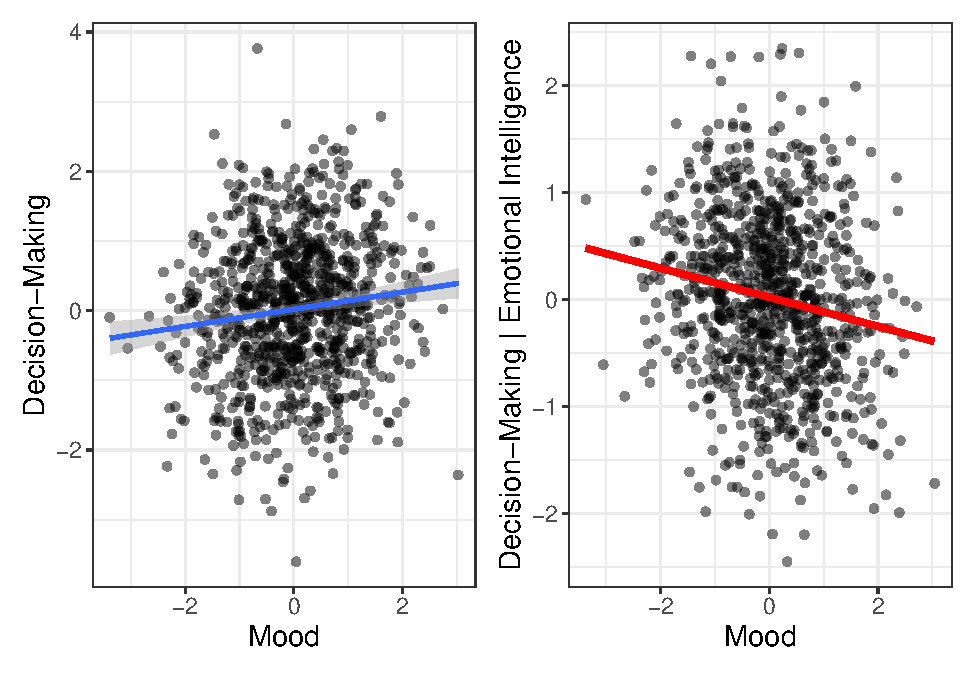
\includegraphics{visual_partitions_files/figure-latex/mainEffects-1.pdf}
\caption{\label{fig:mainEffects}This figure shows a simple bivariate relationship between mood and decision-making (left) and a partial residual plot (right). The simple bivariate correlation suggests a simple positive relationship between mood and decision-making, but the multivariate (conditional) relationship shows that, once we control for emotional intelligence, the relationship between mood and decision-making is actually negative. In other words, we have a ``suppressor'' effect.}
\end{figure}

When using a multivariate model, a simple bivariate graphic may be misleading because it shows the ``total effect'' of the bivariate relationship. This total effect ignores the multivariate nature of the data. When these same effects are plotted as PRPs, it subtracts out the effect of the covariate and displays the net effect of the variable of interest. The net effect may be very different from that shown by a simple bivariate plot. For this reason, the first rule of visual partitions is to \textbf{plot conditional effects using partial residual plots}.

However, we need not plot both variables simultaneously (e.g., using flexplot to visualize one variable on the \(X\)-axis and the other paneled). The reason for this is because the effect of the variable of interest (in this case, mood) does not depend on specific values of the other variable, because there are no interactions. Rather, it only depends on the \emph{average} value of the other variable, which is why we can plot the main effects with a simple partial residual plot.

\subsection{When the ``True Model'' Contains Nonlinear Effects}\label{when-the-true-model-contains-nonlinear-effects}

Now suppose the true model contains one or more nonlinear effects. Returning to the suicide ideation dataset, maybe we are interested in modeling the effects of stress and health on suicide ideation. Recall that there is a nonlinear effect of stress on suicide ideation. If we were to plot a PRP of the linear effect of stress (left image in Figure \ref{fig:nonlinear}), that visual would be misleading. (In this case, the nonlinear stress effect is very striking, so we would likely notice the problem with our visual). These results highlight the second rule of visual partitions: \textbf{when nonlinear effects exist, we must plot both the linear and nonlinear terms of that variable simultaneously.} Beyond that, however, we can plot this variable with a simple bivariate PRP.

\begin{figure}
\centering
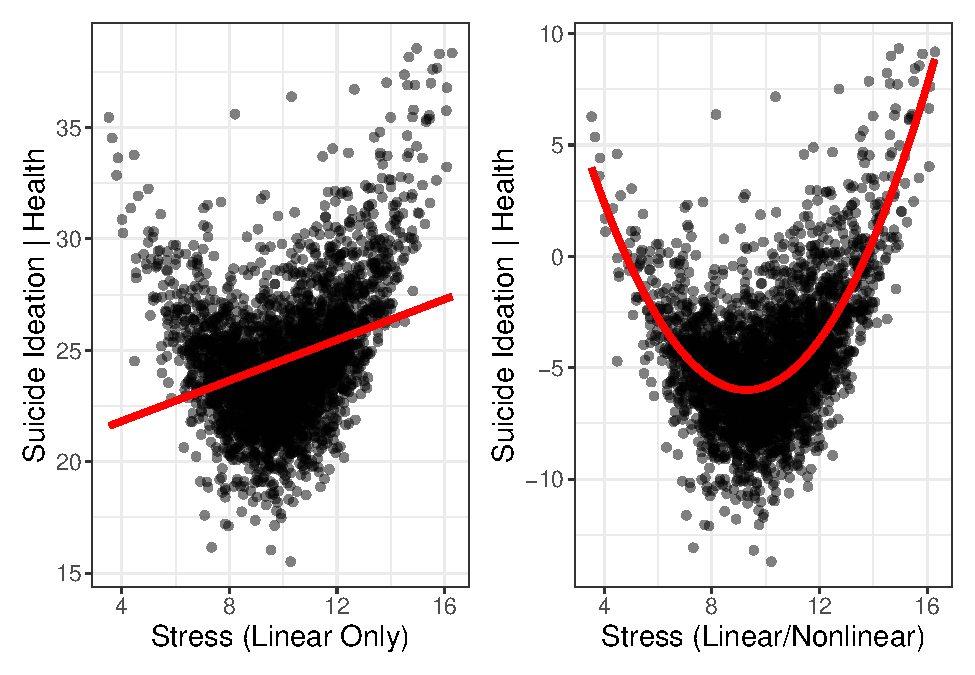
\includegraphics{visual_partitions_files/figure-latex/nonlinear-1.pdf}
\caption{\label{fig:nonlinear}This figure shows PRPs of the stress/suicide ideation relationship (after controlling for health). The left plot shows the relationship between stress and suicide ideation (after controlling for health), while overlaying a regression line. The fit from this graphic is misleading since stress has a nonlinear effect. The right plot shows the linear and nonlinear effects.}
\end{figure}

\subsection{When the ``True Model'' Contains Interaction Effects}\label{when-the-true-model-contains-interaction-effects}

Now suppose the ``true model'' contains interaction effects. It is generally known that one should not interpret main effects in the presence of interactions (Appelbaum \& Cramer, 1974), since the size (and sometimes the direction) of the main effect differs depending on the level of the variable with which it interacts (as with our vultures and rot example). Put differently, the interpretation of one variable's effect is ``entangled'' with the other variable's values. For this reason, all variables involved in the interaction \emph{must} be visualized together.

Consider Figure \ref{fig:interactionPrp}, which shows the relationship between ideation and depression (on the left) and ideation with depression/friend ideation (on the right). The left plot would lead us to believe that increases in depression always increase suicide ideation. However, the plot on the right reveals that the relationship is more complex--it depends on the suicide ideation of one's friend.

\begin{figure}
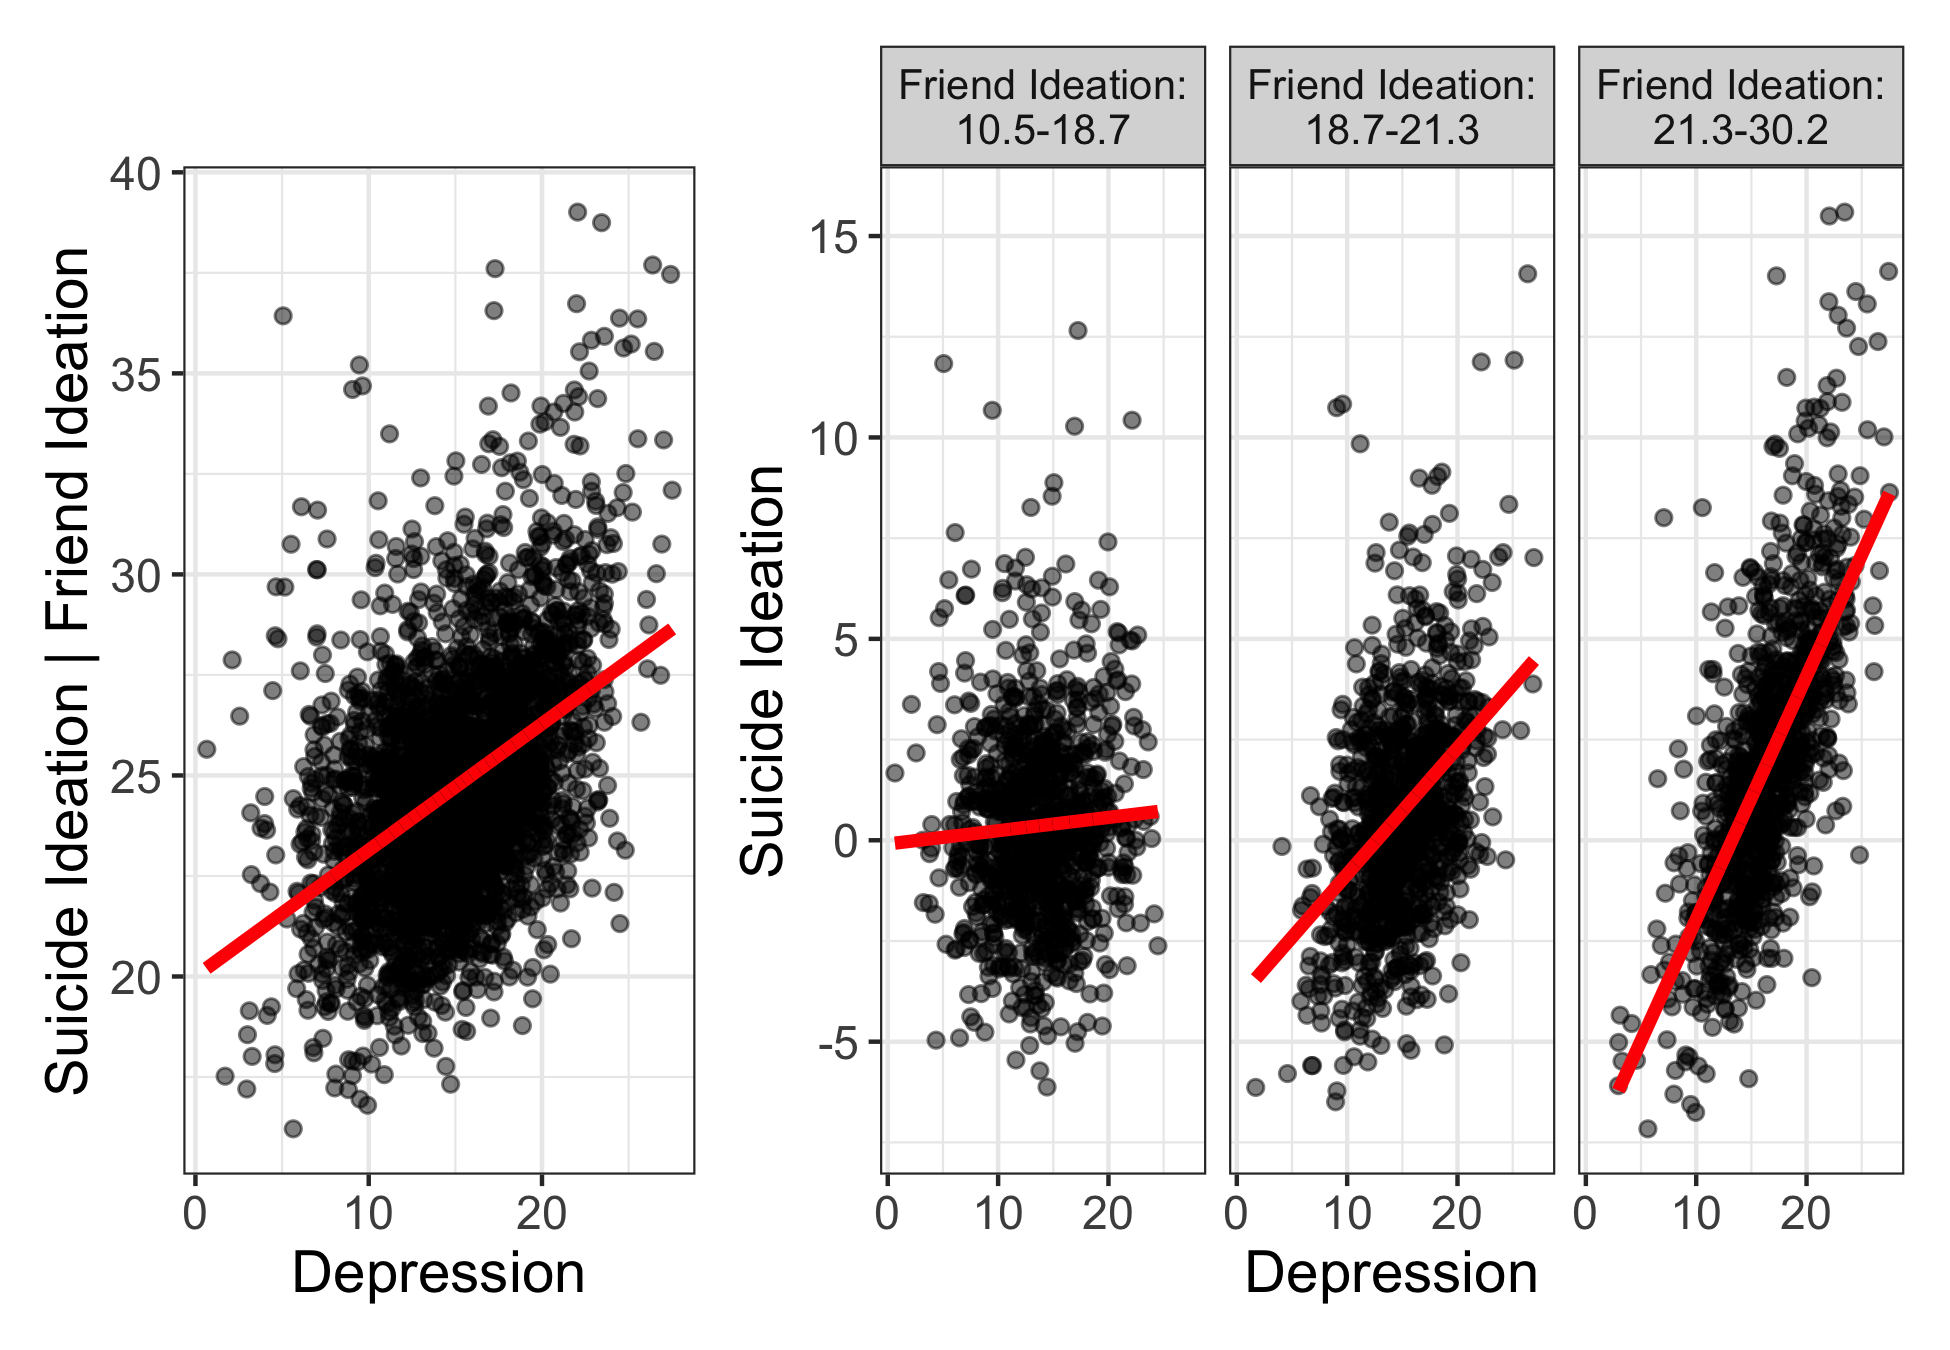
\includegraphics[width=0.9\linewidth]{visual_partitions_files/figure-latex/interactionPrp-1} \caption{This figure shows PRPs of the depression/ideation main effect (on the left) and the depression/friend ideation interaction (on the right). The figure on the left is misleading as it suggests more depression increases ideation. The right figure clarifies this relationship.}\label{fig:interactionPrp}
\end{figure}

This leads us to the third rule of visual partitions: \textbf{variables which interact must be visualized together}. This applies to not only two-way interactions, but three-way, four-way, etc. interactions. However, these variables that interact can be interpreted in relative isolation (provided one uses a PRP to condition for the other variables in the model). For example, we need only visualize depression/friend ideation together, but need not include stress in our interpretation, except through residualizing it.

\subsection{Summary of the Rules for Visual Partitions}\label{summary-of-the-rules-for-visual-partitions}

In summary, for visual partitions to be valid interpretations of the multivariate model, we must obey the following rules:

\begin{enumerate}
\def\labelenumi{\arabic{enumi}.}
\tightlist
\item
  Variables with main effects should be interpreted with PRPs
\item
  For variables containing nonlinear terms, both the linear and nonlinear effects should be visualized together with PRPs
\item
  Variables that interact with one another must be visualized together in a PRP
\end{enumerate}

Provided we follow these rules, the end result of a visual partitioning analysis will be a simple graphic that conveys the entirety of the multivariate model without bias. Furthermore, each individual plot can be interpreted in isolation, without fear of missing critical components of the multivariate model.

For example, suppose our ``true model'' for the ideation dataset is as follows:

\begin{align}
\label{eq:model} \text{suicide ideation}=b_0 +& b_1 \text{health} \\
\nonumber                              +& b_2 \text{stress} + b_3 \text{stress}^2 \\
\nonumber                              +& b_4 \text{friend ideation} + b_5 \text{depression} + b_6 \text{friend ideation} \times \text{depression} 
\end{align}

To provide a complete representation of the entire multivariate model requires only three plots: (1) a bivariate PRP of the linear health relationship, (2) a bivariate plot of the linear/nonlinear stress relationship, and (3) a multivariate plot of depression/friend ideation. Each of these plots can be interpreted in isolation without bias.

\subsection{Visual Partitions and Linear Model Assumptions}\label{visual-partitions-and-linear-model-assumptions}

Recall that linear models make a few key assumptions:

\begin{enumerate}
\def\labelenumi{\arabic{enumi}.}
\tightlist
\item
  Normality (meaning that the residuals of the model must be normally distributed)
\item
  Homoscedasticity (meaning that the size of the residuals do not drastically fluctuate across the values of the predictors)
\item
  Independence.
\item
  Additivity.
\end{enumerate}

This last assumption is not often talked about and is, perhaps, poorly understood. This assumption states that all modeled main effects contain only simple effects. In other words, if there are main effects in the hypothesized model, this assumption states that these variables do not have nonlinear effects, nor do they interact with one another (Gelman \& Hill, 2006). The reason for this last assumption is clear: if there are nonlinear and/or interactive effects, any interpretation of the main effects is misleading. Likewise, visualizing main effects when they have non-additive effects is misleading. As such, the rules of visual partitions are implied by the assumptions of linear models.

\section{Visual Partitions in Confirmatory Versus Exploratory Research}\label{visual-partitions-in-confirmatory-versus-exploratory-research}

Now that I have introduced the appropriate tools and identified the rules for visual partitions, let us now turn to how they can be practically applied in research settings. Before I do so, it is important to discuss the distinction between confirmatory and exploratory research. This is important because visual partitions play different roles in confirmatory versus exploratory research.

The rules for conducting confirmatory research are quite strict (Fife \& Rodgers, in press; Wagenmakers, Wetzels, Borsboom, Maas, \& Kievit, 2012). The reason for this is because confirmatory research relies strongly on the rules of probability. For probability estimates (e.g., \(p\)-values and confidence intervals) to have probabilistic meaning, the following conditions must be met:

\begin{itemize}
\tightlist
\item
  The sample size, Type I/II error rates, and exact model must be specified in advance
\item
  Only one hypothesis test can be performed (or probability estimates must be corrected for multiple comparisons)
\item
  There can be no deviation from the original model/sample size plan
\item
  The assumptions of the model must be met
\end{itemize}

(We might also add that confirmatory research will most likely be preregistered.)

When one is doing strict confirmatory research (which is quite rare), visual partitions are used primarily to \emph{communicate} or present the multivariate model. They are a succinct representations of a complex multivariate model. This representation is far more informative than a simple ANOVA summary table. In other words, the ``strategy'' for confirmatory research is to simply produce a PRP using the aforementioned three rules. However, these visual partitions might also indirectly play a \emph{diagnostic} role simply because these visuals may highlight nonlinearities a main effects model failed to capture. If this is the case, the analysis is no longer confirmatory and migrates to exploratory (or ``rough confirmatory'', Fife \& Rodgers, 2022).

Rough confirmatory research occurs when one has specified a hypothesis in advance, but has not prespecified the statistical model. As such, researchers might have the flexibility to audition different measures of the outcome variable and/covariates, model interactions and/or nonlinear effects, perform transformations, etc. This might sound like ``p-hacking'' (Simmons, Nelson, \& Simonsohn, 2011). However, there's a critical (but small) difference between p-hacking and rough confirmatory research: rough confirmatory research is transparent, while p-hacking is not. It has been argued that most research is exploratory (McArdle, 2012), or at most rough confirmatory (Fife \& Rodgers, 2022).

With rough confirmatory/exploratory research, the goal shifts from \emph{communicating} multivariate effects to \emph{identifying} multivariate effects, including (and especially) interaction and nonlinear effects.\footnote{It is common knowledge that \(p\)-values are susceptible to ``p-hacking,'' or multiple testing. It can be argued that searching for striking results in plot after plot is not any different than searching for statistically significant results (Buja et al., 2009). In a sense, this is true. However, the \(p\)-value is supposed to indicate the probability of observing the data (or data more extreme) given that the null is true. When doing multiple testing, this \(p\)-value no longer means what it's supposed to mean; multiple testing has rendered the \(p\)-value uninterpretable (in any probablistic sense). For visuals, on the other hand, the plots do not rely on probabilities and their interpretation doesn't change when one has done multiple testing. However, there is still the possibility that patterns uncovered through visualizations are spurious. Consequently, one should confirm these patterns on a fresh dataset.} In the following section, we will identify a strategy for using the idea of visual partitions to uncover hidden patterns in data.

\subsection{Overall Strategy for Visual Partitioning in Exploratory/Rough Confirmatory Research}\label{overall-strategy-for-visual-partitioning-in-exploratoryrough-confirmatory-research}

Research questions (and hypotheses) will specify the appropriate outcome and predictor variable(s). Naturally, one might begin by assuming a simple main-effects model. To identify the viability of a main-effects-only model, one can combine the aforementioned tools into a simple strategy. The goal of this strategy is to visually partition the results of a multivariate analysis and to ensure additivity is met. The strategy consists of five steps:

\begin{enumerate}
\def\labelenumi{\arabic{enumi}.}
\tightlist
\item
  Identify nonlinear effects with loess lines.
\item
  Identify interactions with marginal plots.
\item
  Model (and optionally test) for nonlinear/interactive effects found in Step 2.
\item
  Use PRPs to perform residual analysis from the model in Step 3.
\item
  Visualize final model partitions using PRPs.
\end{enumerate}

Each of these steps requires some elaboration, which we do in the next sections.

\subsubsection{1. Identify Nonlinear Effects}\label{identify-nonlinear-effects}

This step is, perhaps, the easiest. This step requires the researcher to produce a simple bivariate graphic of each variable against the outcome variable. Flexplot will default to plotting a loess line. If the line has a pattern of nonlinearity for a particular variable, a nonlinear term may need to be added to the model.

At first glance, this strategy seems prone to bias; are we not ignoring the multivariate nature of the data if we simply plot bivariate scatterplots? For example, a nonlinear effect might appear to exist in a bivariate graphic, but disappears once we've modeled an interaction effect. Or, conversely, the bivariate plot might suggest a variable's effect is linear, but when viewed in the context of other variables, there is a nonlinear effect.

Each of these scenarios are possible. However, we have several steps that remain that are designed to detect any sort of effects we might miss in the earlier stages. By beginning with simple bivariate plots, it gives us a straightforward starting point.

\subsubsection{2. Identify Interaction Effects With Marginal Plots}\label{identify-interaction-effects-with-marginal-plots}

Once we have identified plausible nonlinear effects, it is time to identify interactions. Recall that Flexplot allows one to visualize multiple variables simultaneously, using symbols/lines/colors and/or panels. The purpose of visualizing these simultaneously is to detect interactions. However, unless the user displays one of the variables doing the interacting on the \(X\)-axis, and unless the other variable doing the interacting is displayed somewhere else in the Flexplot graphic, they cannot be visually detected. As such, Step \#2 is an iterative process.

For our example data, we would alternate placing friend ideation, health, stress, and depression on the \(X\)-axis. Recall that depression interacts with friend ideation. To detect this interaction, friend ideation \emph{or} depression must be on the \(X\)-axis, and the other variable must be displayed as separate lines/colors/symbols or in separate panels. However, marginal plots will only be able to reveal nonparallel lines in the variables represented as row/column panels. So, the following Flexplot equations would detect the interaction:

\begin{itemize}
\tightlist
\item
  \texttt{flexplot(ideation\textasciitilde{}depression\ \textbar{}\ health\ +\ friend\_ideation,\ data=ideation)} (slopes would vary as a function of row panels)
\item
  \texttt{flexplot(ideation\textasciitilde{}friend\_ideation\ +\ stress\ \textbar{}\ depression\ +\ health,\ data=ideation)} (slopes would vary as a function of column panels)
\item
  \texttt{flexplot(ideation\textasciitilde{}depression\ +\ friend\_ideation\ \textbar{}\ health,\ data=ideation)} (slopes would vary as a function of colors/symbols/lines, though the marginal plots wouldn't help detect these interactions)
\end{itemize}

On the other hand, the following Flexplot equations would \emph{not} detect interactions:

\begin{itemize}
\tightlist
\item
  \texttt{flexplot(ideation\textasciitilde{}health\ \textbar{}\ depression\ +\ friend\_ideation,\ data=ideation)} (neither interacting variable is on the \(X\)-axis)
\item
  \texttt{flexplot(ideation\textasciitilde{}depression\ \textbar{}\ stress\ +\ health,\ data=ideation)} (one of the interacting variables {[}friend ideation{]} isn't displayed)
\end{itemize}

Once again, we emphasize this is an iterative process: one must take turns visualizing each variable on the \(X\)-axis, and one must allow every other variable in the model to be in a panel at one time or another. This may require several plots.

There is one important caveat. Often, predictor variables are correlated with one another. For this reason, sometimes a variable that doesn't actually interact with the variable on the \(X\)-axis will reveal nonparallel lines when, in fact, the lines are nonparallel only because that variable is correlated with another variable with which it interacts. In these situations, it is best to identify the variable with the strongest evidence of nonparallel lines, model that, then use PRPs to see if any remaining variables contain interactions.

\subsubsection{3. Model Nonlinear/Interaction Effects}\label{model-nonlinearinteraction-effects}

Step \#1 will be helpful in identifying nonlinear effects, while Step \#2 will help in identifying interactions. Once they are identified, these effects should be entered into a linear model.

One of the weaknesses of visualizations is their ambiguity.(Though, of course, ambiguity is also a strength, at least when ambiguity is merited, Fife, 2020). It is difficult to determine from a simple graphic whether a curvilinear effect is nonlinear \emph{enough} or if slopes are not parallel \emph{enough} to warrant modeling them. This is where non-visual statistics come in.

We favor a model comparison approach (Rodgers, 2010). With this approach, one specifies a ``full model,'' which contains the multiplicative effect (e.g., a quadratic term) and a ``reduced model'' (e.g., a model with main effects only). Once specified, these two models can be compared (e.g., using the \texttt{anova} function in R, or the \texttt{model.comparison} function in \texttt{flexplot}). The \texttt{model.comparison} function will report AIC, BIC, Bayes factors, \(p\)-values, and \(R^2\). These statistics can assist users in deciding whether the multiplicative effects are worth keeping.

Ideally, by the end of this step, the user has a good idea of what model is most appropriate. The next step will assist in ensuring no important effects have been missed.

\subsubsection{4. Visualize Residuals Using PRPs}\label{visualize-residuals-using-prps}

Recall that PRPs are a visual representation of the effect of the variable(s) of interest on the outcome, after controlling for one or more covariates. Another way to think about controlling (or conditioning) is ``subtraction.'' When we condition on one or more effects, we are \emph{subtracting} out the effects of those variables. Presumably, when we subtract a variable's effect from the outcome, that same variable should no longer be associated with that outcome. We \emph{should} see a flat relationship between the variable and the residuals if all effects have been modeled. If, on the other hand, that variable has a multiplicative effect and we have only modeled the additive effect, we should still see a relationship between the variable of interest and the residuals of the model. This is exactly what happened in Figure \ref{fig:missingnonlin}.

We can use this fact to determine whether the effects we've modeled are unbiased. After the nonlinear/quadratic effects are identified (from Steps 1/2) and modeled (from Step 3), we then use PRPs in much the same we way used marginal plots in Step 2; we sequentially plot the residuals against each variable on the \(X\)-axis (and the remaining variables in panels or as colors/lines/symbols) and look for flat slopes. If they're all flat and nonlinear, we have captured all signal in the model. If not, there may be missing two-way or three-way interactions, or additional nonlinear terms.

As an example, consider Figure \ref{fig:threeway}. In this example, we have simulated the data to contain both a two-way and a three-way interaction, but have only modeled the two-way interaction. The red lines are the model-implied fitted lines, while the blue lines are regression lines. (We can add regression lines to any PRP by adding the \texttt{method="lm"} argument). The partial residual plot reveals that we \emph{still} have nonparallel slopes, even after we've subtracted out the main effects and the two-way interaction, at least in some regions of the Flexplot graphic. These results suggest there's an unmodeled three-way interaction.

\begin{figure}

{\centering 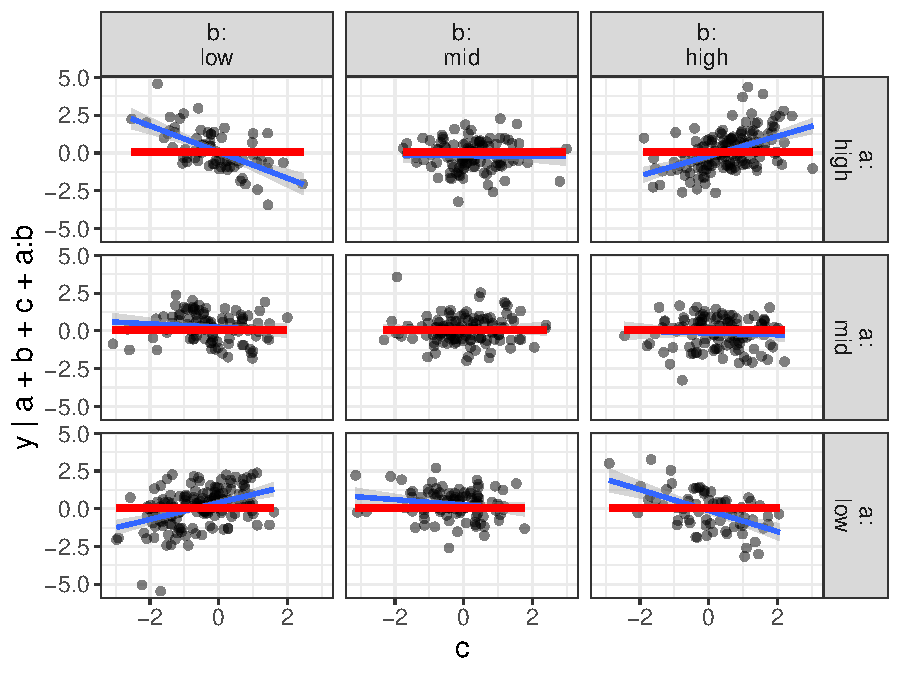
\includegraphics[width=0.7\linewidth]{visual_partitions_files/figure-latex/threeway-1} 

}

\caption{This plot shows a PRP where the user has modeled a two-way interaction, but there's an unmodeled three-way interaction present. Here, the red lines show the model-implied fit, while the blue lines show regression lines. The blue lines suggest there's still some signal remaining that hasn't been modeled.}\label{fig:threeway}
\end{figure}

\subsubsection{5. Visualize the Final Model Using PRPs}\label{visualize-the-final-model-using-prps}

While we have written the previous sections sequentially, in actuality, this is an iterative process. However, once all PRPs show relatively flat lines across all variables, it is time to visualize the final model using conditionally independent partitions. To do so, we follow the same rules for confirmatory visual partitions (using PRPs we visualize main effects with bivariate plots, visualize nonlinear effects with their linear effects, and visualize interacting variables together).

Of course, for each of these PRPs, the final model will be inputted into the \texttt{partial\_residual\_plot} function. Also, the \texttt{added\_term} argument should contain every term in the linear model associated with the variable(s) of interest. For example, any variables with only main effects would simply have the main effect as the \texttt{added\_term} argument (e.g., \texttt{\textasciitilde{}health}). For nonlinear terms, we would add both the linear and nonlinear terms to the \texttt{added\_term} argument (e.g., \texttt{\textasciitilde{}stress\ +\ I(stress\^{}2)}). For interaction effects, we add both the variable of interest as well as all other variables that it interacts with (e.g., \texttt{\textasciitilde{}\ depression\ +\ friend\_ideation\ +\ depression:friend\_ideation}). For our suicide ideation dataset, our PRP code might look like this:

\begin{Shaded}
\begin{Highlighting}[]
\CommentTok{\# fit the final model}
\NormalTok{final\_model }\OtherTok{=} \FunctionTok{lm}\NormalTok{(ideation}\SpecialCharTok{\textasciitilde{}}\NormalTok{health }\SpecialCharTok{+} \CommentTok{\#main effect of health}
\NormalTok{    stress }\SpecialCharTok{+} \FunctionTok{I}\NormalTok{(stress}\SpecialCharTok{\^{}}\DecValTok{2}\NormalTok{) }\SpecialCharTok{+} \CommentTok{\# nonlinear effect of stress}
\NormalTok{    depression }\SpecialCharTok{*}\NormalTok{ friend\_ideation, }\CommentTok{\# interaction effect}
    \AttributeTok{data=}\NormalTok{ideation)}

\CommentTok{\# plot the health effect}
\FunctionTok{partial\_residual\_plot}\NormalTok{(ideation}\SpecialCharTok{\textasciitilde{}}\NormalTok{health, }
              \AttributeTok{model=}\NormalTok{model, }
              \AttributeTok{added\_term =} \SpecialCharTok{\textasciitilde{}}\NormalTok{health, }
              \AttributeTok{data=}\NormalTok{ideation)}

\CommentTok{\# plot the nonlinear stress effect}
\FunctionTok{partial\_residual\_plot}\NormalTok{(ideation}\SpecialCharTok{\textasciitilde{}}\NormalTok{stress, }
              \AttributeTok{model=}\NormalTok{model, }
              \AttributeTok{added\_term =} \SpecialCharTok{\textasciitilde{}}\NormalTok{stress }\SpecialCharTok{+} \FunctionTok{I}\NormalTok{(stress}\SpecialCharTok{\^{}}\DecValTok{2}\NormalTok{), }
              \AttributeTok{data=}\NormalTok{ideation) }

\CommentTok{\# plot the interaction effect}
\FunctionTok{partial\_residual\_plot}\NormalTok{(ideation}\SpecialCharTok{\textasciitilde{}}\NormalTok{friend\_ideation }\SpecialCharTok{|}\NormalTok{ depression, }
                      \AttributeTok{model=}\NormalTok{model, }
                      \AttributeTok{added\_term =} \SpecialCharTok{\textasciitilde{}}\NormalTok{depression}\SpecialCharTok{*}\NormalTok{friend\_ideation, }
                      \AttributeTok{data=}\NormalTok{ideation) }
\end{Highlighting}
\end{Shaded}

The above code would produce the visual partitions we see in Figure \ref{fig:allplotstogether}. (Note: the actual code used to produce these plots are slightly different than what is displayed because we wanted to have more intuitive labels than what PRPs naturally produce).

\begin{figure}

{\centering 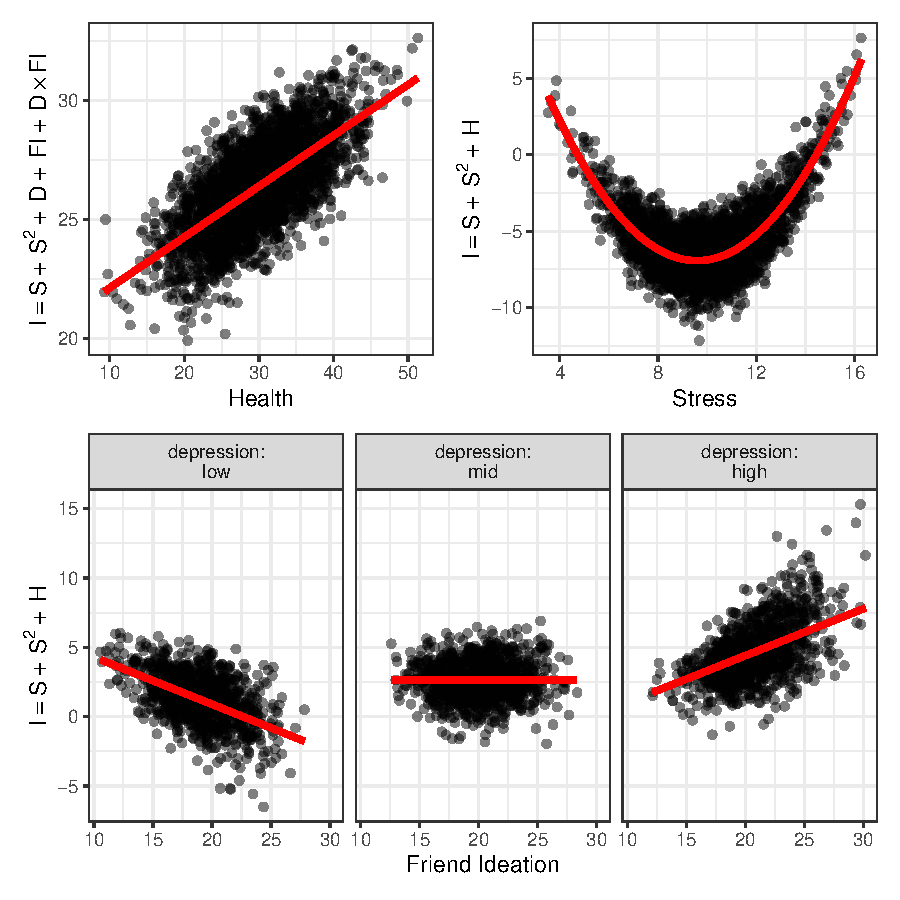
\includegraphics[width=0.75\linewidth]{visual_partitions_files/figure-latex/allplotstogether-1} 

}

\caption{The entire multivariate model in Equation 1 can be visualized using only three PRPs. The top-left plot shows the health effect, the top-right plot shows the stress nonlinear effect, and the bottom plot shows the depression/friend ideation interaction.}\label{fig:allplotstogether}
\end{figure}

\section{Example Analyses}\label{example-analyses}

For our applied analysis, we're going to base our analysis loosely on a study done by Yang, Fu, Chen, Hsieh, and Lin (2019). Their paper sought to determine the relationship between depression (measured by CESD), Internet addiction (measured by the Internet Addiction Test, or IAT), and health (measured by Health Promoting Lifestyle Profile, or HPLP). More specifically, we will investigate the influence of health and Internet addiction on depression, after controlling for age, BMI, smoking status, alcohol drinking status, and religion.

A naive analysis of these data might look like Table \ref{tab:anovatab2}. This analysis suggests Internet addiction, health, and drinking have statistically significant effects. However, as we shall see, this conclusion may be premature and misleading.

\begin{table}[tbp]

\begin{center}
\begin{threeparttable}

\caption{\label{tab:anovatab2}Naive Analysis of the Relationship Between Health/Internet and CESD, After Controlling for Age, BMI, Drinking, Smoking, and Religion}

\begin{tabular}{lccccc}
\toprule
 & DF & SS & MS & F & p\\
\midrule
Health & 1 & 495.42 & 495.42 & 7.85 & 0.005\\
Internet & 1 & 5,997.56 & 5,997.56 & 95.03 & <0.001\\
Age & 1 & 72.84 & 72.84 & 1.15 & 0.283\\
BMI & 1 & 140.61 & 140.61 & 2.23 & 0.136\\
Drinking & 1 & 273.23 & 273.23 & 4.33 & 0.038\\
Smoking & 1 & 24.11 & 24.11 & 0.38 & 0.537\\
Religion & 1 & 19.47 & 19.47 & 0.31 & 0.579\\
Residuals & 495 & 31,240.93 & 63.11 &  & \\
\bottomrule
\end{tabular}

\end{threeparttable}
\end{center}

\end{table}

For the analyses that follow, we transformed CESD and health using a square root transformation. This not only rendered the residuals of the model more normally distributed, but it also addressed some initial problems with heteroscedasticity.

\subsection{1. Visualize Multiple Predictor Variables Simultaneously}\label{visualize-multiple-predictor-variables-simultaneously}

As mentioned previously, this step requires us to plot each predictor variable (in our case, age, BMI, smoking status, alcohol, religion, HPLP, and Internet addiction) on the \(X\)-axis in order to investigate nonlinear effects. I chose to \emph{not} reproduce all the plots we generated for our analysis in this paper to save space. Rather, I will provide a sample of some of the most instructive plots.

Initially, none of the bivariate plots showed nonlinear effects. However, I discovered in the next step there was a potential nonlinear \emph{and} interactive effect between Internet/CESD, and either religion or health. Figure \ref{fig:applied1} shows a plot of the relationship between Internet addiction and CESD, for health and religion. The initial plots with loess lines (not shown) indicated a curvilinear effect. For that reason, Figure \ref{fig:applied1} plots quadratic regression lines. It also seems the effect of Internet on depression may depend on one or more of these variables (i.e., there may be an interaction present). We will investigate this further in the next section.

\begin{figure}

{\centering 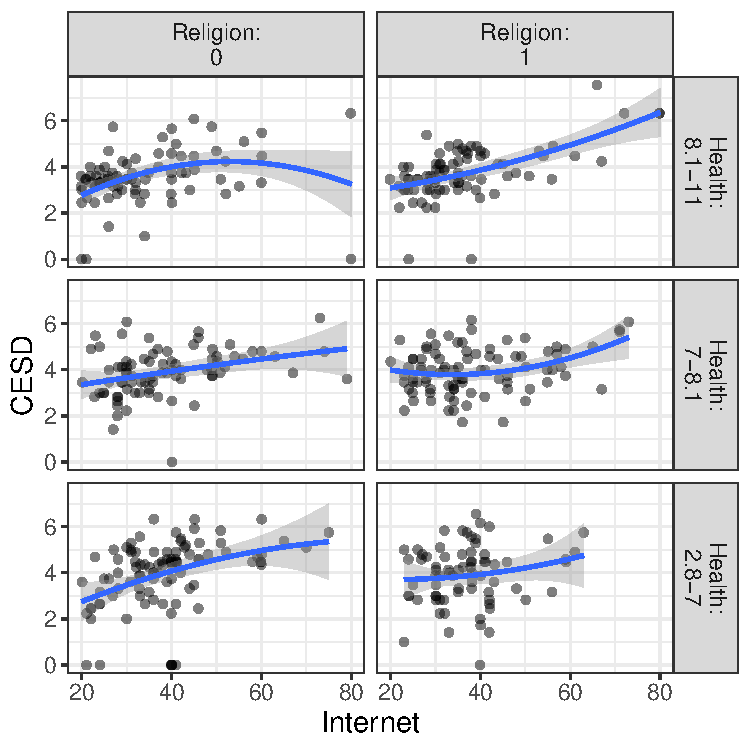
\includegraphics[width=0.75\linewidth]{visual_partitions_files/figure-latex/applied1-1} 

}

\caption{Flexplot visual of the relationship between Internet addiction and CESD, for various ages and levels of religion. The plots indicate some nonlinearity and possible interaction effects.}\label{fig:applied1}
\end{figure}

\subsection{2. Identify Interaction Effects With Marginal Plots}\label{identify-interaction-effects-with-marginal-plots-1}

Figure \ref{fig:applied2} plots the same image in Figure \ref{fig:applied1}, but with marginal plots. These images suggest the Internet effect is generally positive for each of the levels of health. Across religion, there may be evidence of a small interaction effect; the relationship is concave upward for those who are religious, while it's concave downward for those who are not religious.

\begin{figure}

{\centering 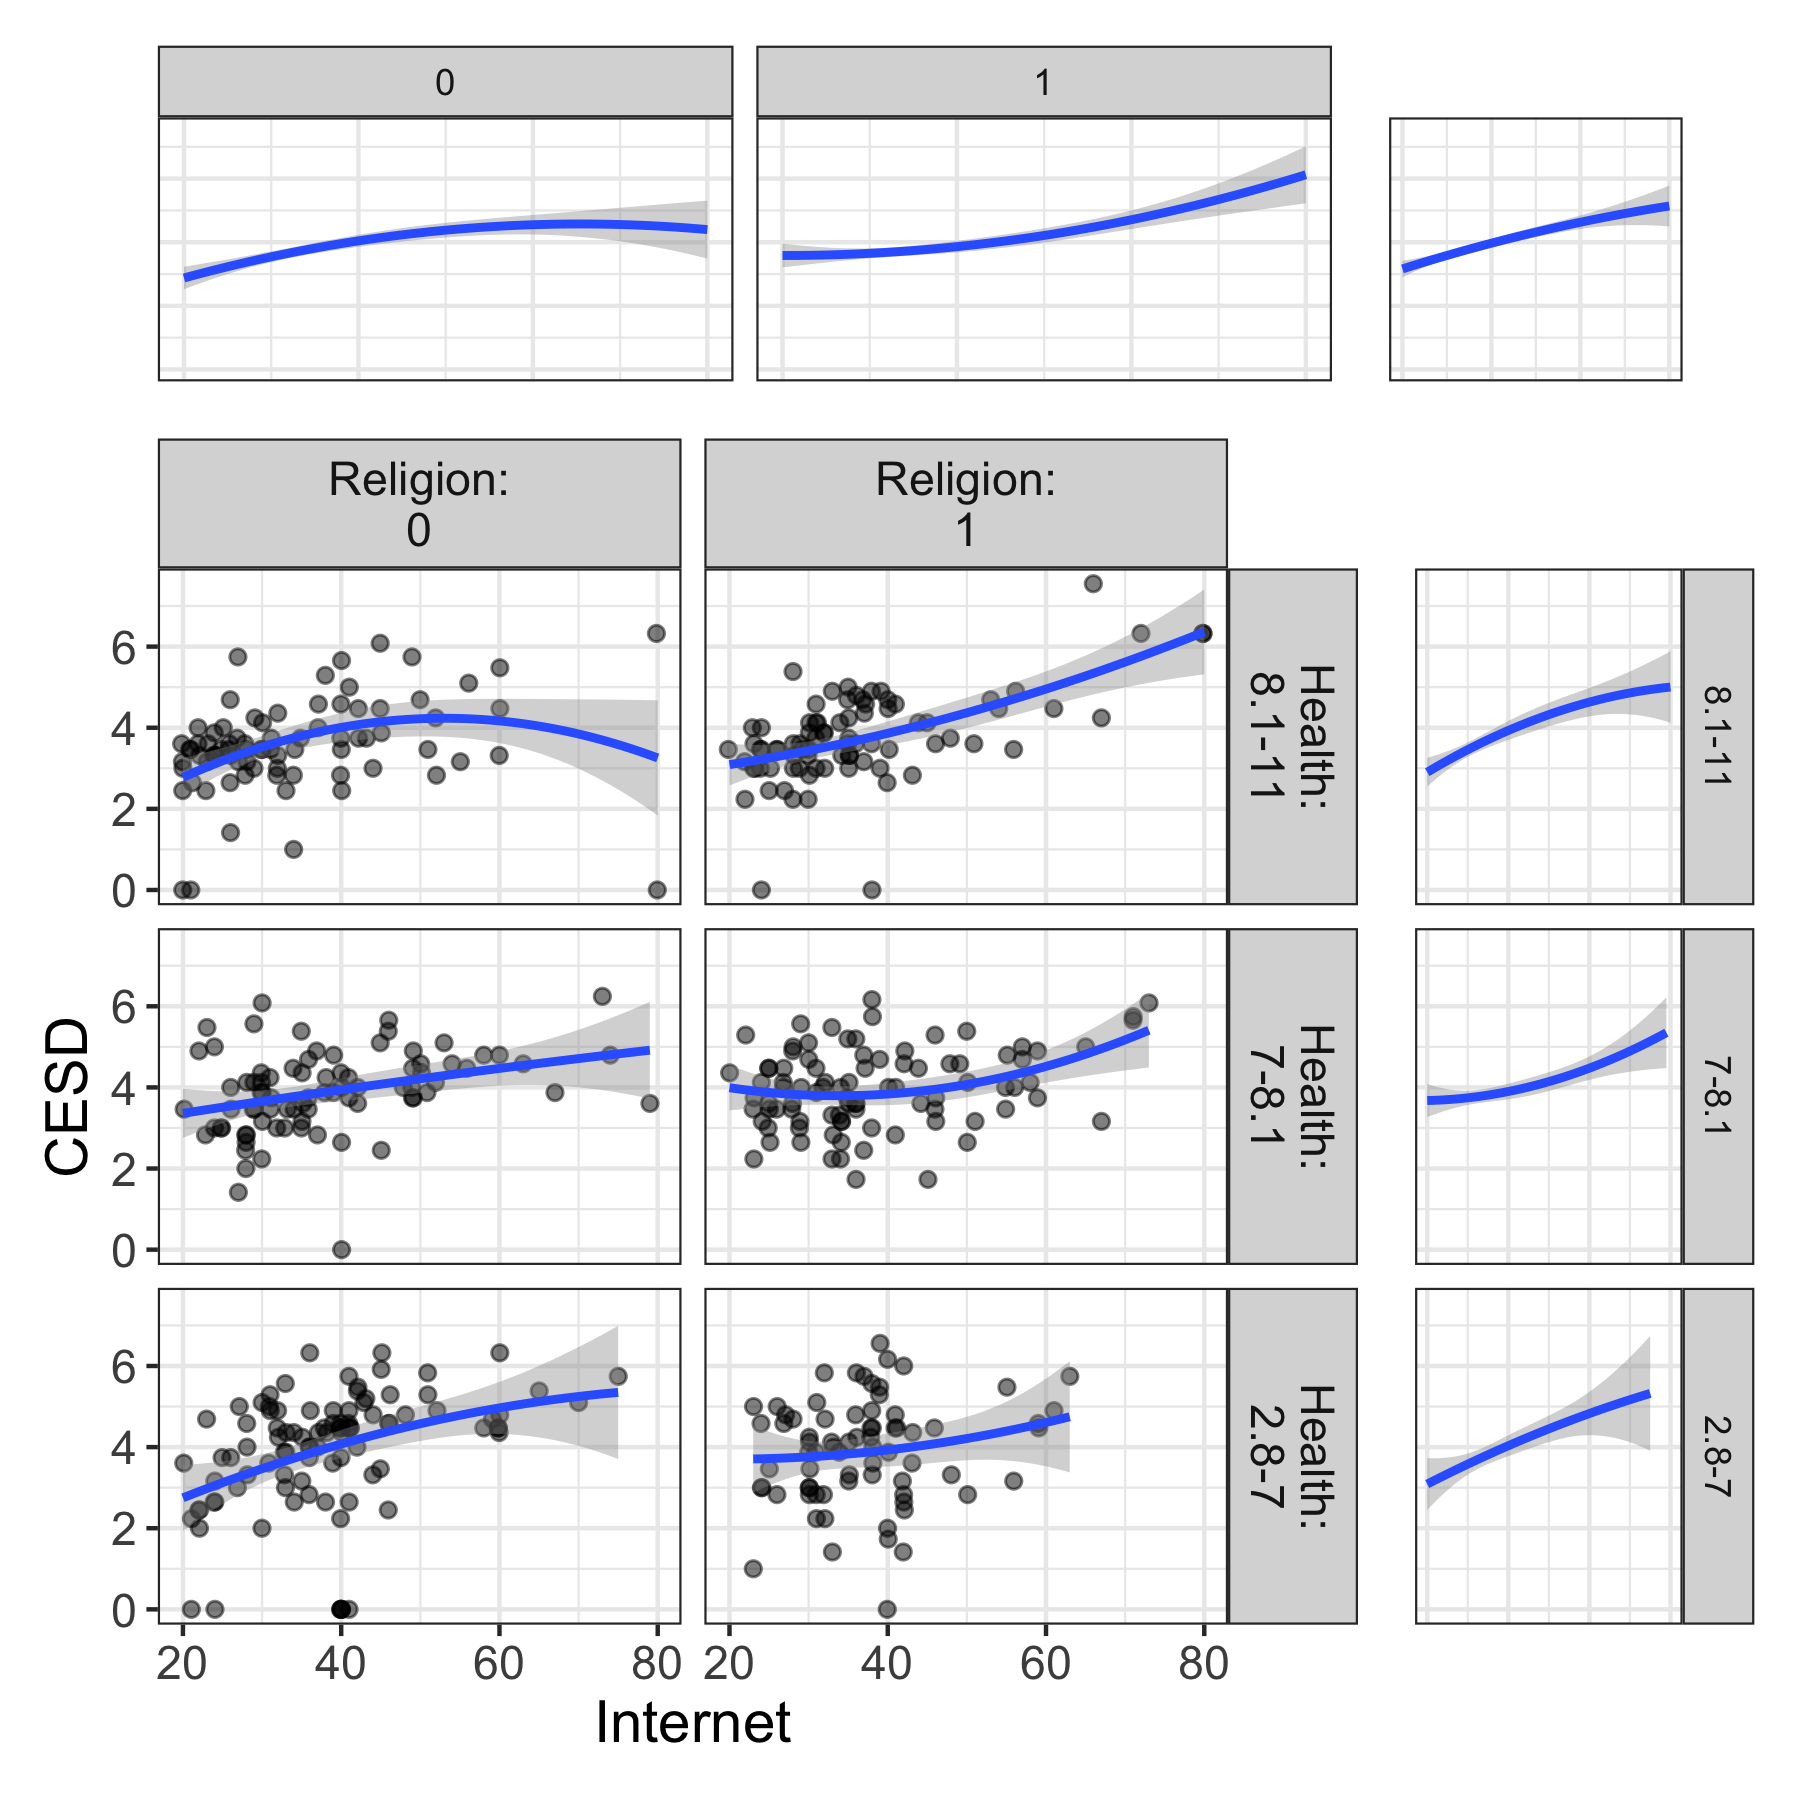
\includegraphics[width=0.75\linewidth]{visual_partitions_files/figure-latex/applied2-1} 

}

\caption{Marginal plot of the relationship between Internet addiction and CESD, for various ages and religion levels. The row marginal plots indicate Internet may interact with religion.}\label{fig:applied2}
\end{figure}

Of course it is difficult to tell conclusively from this graph whether that interaction is worth keeping. To aid in this, we will utilize model comparisons.

\subsection{3. Model Nonlinear/Interaction Effects}\label{model-nonlinearinteraction-effects-1}

Our original model included only main effects of all the variables. These plots suggest we might include nonlinear terms associated with Internet, as well as an interaction with the religion variable.\footnote{The images suggest the interaction manifests itself as a change in the coefficient for the \emph{nonlinear} term (i.e., the quadratic component). For this reason, we need to model both the interaction term between Internet and religion, as well as the interaction between the quadratic term and religion.} To test this, we will utilize model comparisons (Rodgers, 2010). Specifically, we compared the following full and reduced models,

\begin{align}
\nonumber Full\,Model: \text{CESD}    &= Health + Internet + Religion + \\
\nonumber & \qquad Internet \times Religion + Internet^2 + Internet^2 \times Religion \\
\nonumber Reduced\,Model: \text{CESD} &= Health + Internet + Religion \\
\end{align}

(Notice we've omitted several variables that didn't seem to be terribly predictive). We used \texttt{flexplot} to compute the AIC, BIC, the Bayes factor (derived from the BIC), the \(p\)-value from a likelihood ratio test{[}whyp{]}, and the model's \(R^2\). These results are presented in Table \ref{tab:modelcomp}. Unfortunately, the results are a little ambiguous; the AIC and \(p\)-value both favor the full model, while the BIC (and the BF) favor the reduced model. Recall that the BIC is more conservative than the AIC, so the fact that there's disagreement isn't surprising, especially since the full model estimates three additional parameters. Also, the full model explains an additional 2\% of the variance, beyond the reduced model. For the sake of our example, we will accept the full model before moving on to the next section.

\begin{table}[tbp]

\begin{center}
\begin{threeparttable}

\caption{\label{tab:modelcomp}Model Comparison of the Full and Reduced Model for the Depression, Internet Addiction, and Health Dataset.}

\begin{tabular}{lccccc}
\toprule
 & AIC & BIC & BF & p & $R^2$\\
\midrule
Full & 3,516.90 & 3,567.55 & 0.03 & 0.011 & 0.20\\
Reduced & 3,522.29 & 3,560.27 & 38.08 &  & 0.18\\
\bottomrule
\end{tabular}

\end{threeparttable}
\end{center}

\end{table}

\subsection{4. Visualize Residuals Using PRPs}\label{visualize-residuals-using-prps-1}

Having (provisionally) chosen our full model, we will now utilize PRPs to identify whether there are any remaining effects the model has missed. As before, we will only show one representative plot to save space. Figure \ref{fig:prpexample} shows a PRP with Internet on the \(X\)-axis, and health/religion in panels. The residuals of the full model are shown on the \(Y\)-axis. As such, we would expect to see flat lines throughout the plots if we have adequately modeled all effects. We have overlaid loess lines (blue), as well as the model-implied fit (red lines). For the most part, the two lines generate quite similar results, suggesting our model (Full Model) has extracted any signal existing between Internet, health, and religion.

\begin{figure}

{\centering 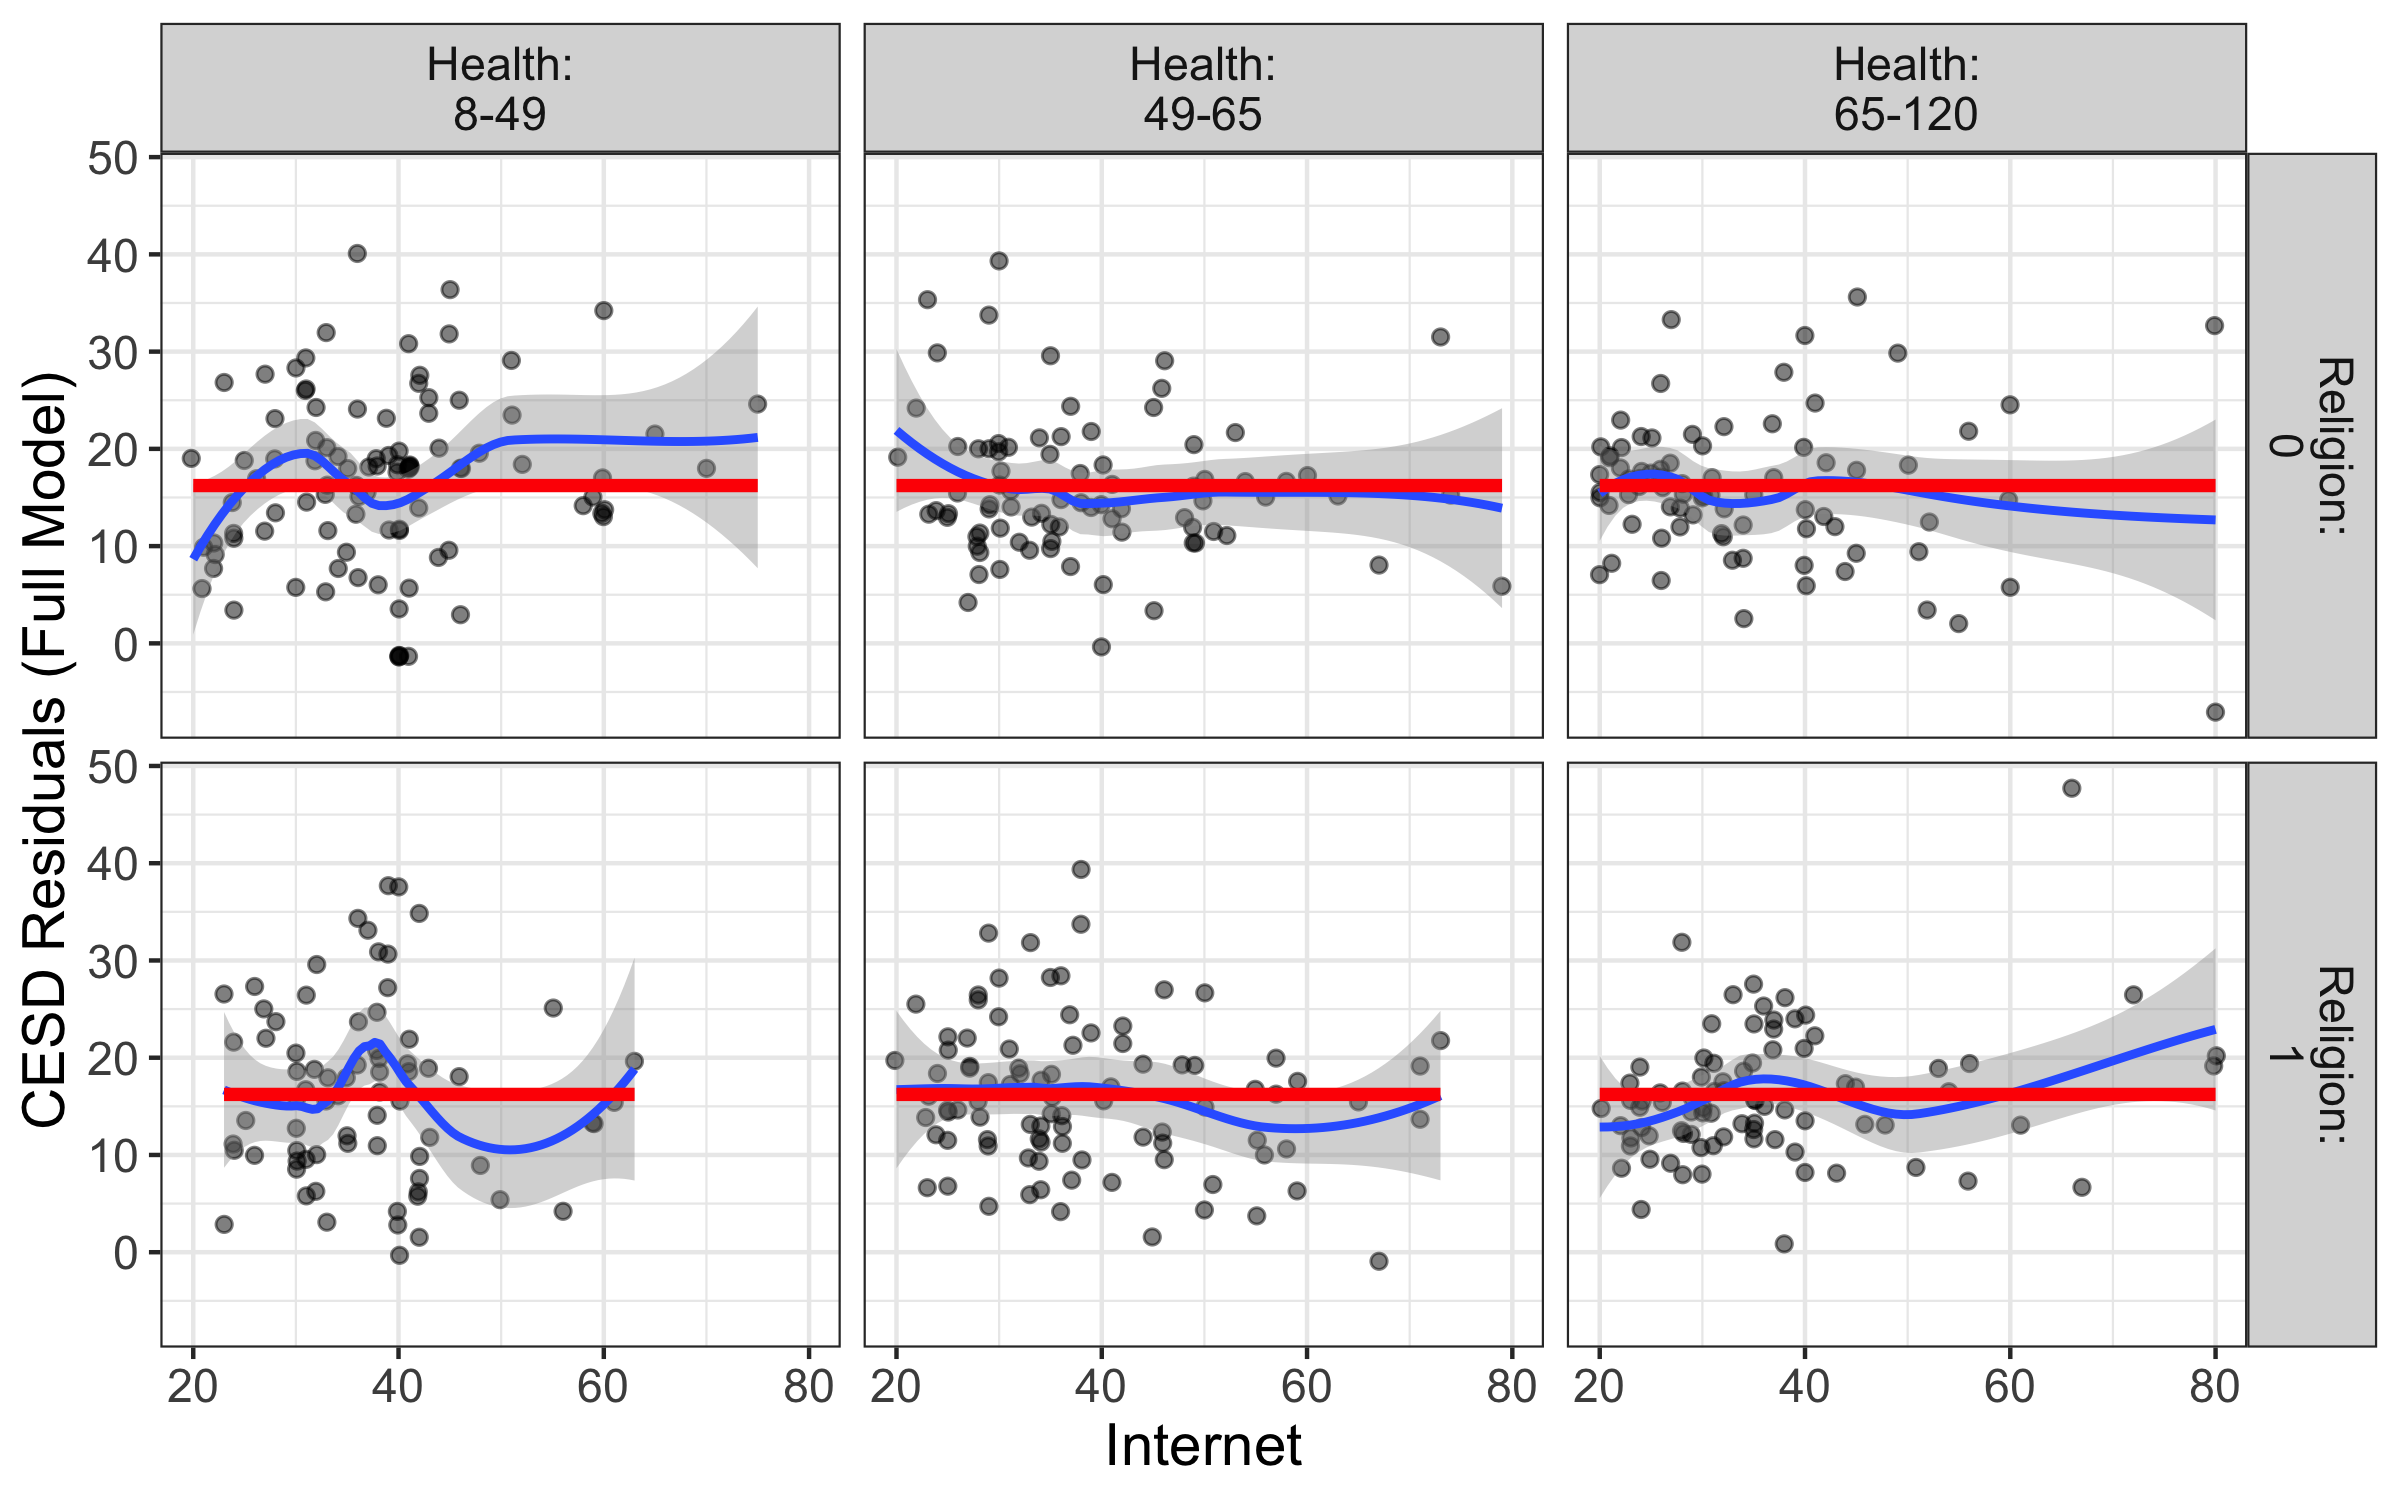
\includegraphics[width=0.75\linewidth]{visual_partitions_files/figure-latex/prpexample-1} 

}

\caption{Partial residual plot between the residuals of CESD for the full model and Internet, health, and religion. Red lines are the model-implied fit and blue lines are loess lines.}\label{fig:prpexample}
\end{figure}

\subsection{5. Visualize the Final Model Using PRPs}\label{visualize-the-final-model-using-prps-1}

Recall that our full model has main effects for all our predictors, as well as a nonlinear effect for Internet and an interaction between the Internet effect and religion. For that reason, our final visualizations should include:

\begin{itemize}
\tightlist
\item
  bivariate plots for BMI, drinking, smoking, age, and health
\item
  a multivariate plot for Internet and religion
\end{itemize}

To save space, we chose not to plot all bivariate plots. Instead, we just plot health, Internet, and religion (since the other variables were covariates and not of theoretical interest). Figure \ref{fig:prpfinalexample} visualizes the marginal effect of health on CESD (top plot) and the marginal effect of Internet/religion (bottom plot). These results suggest there's a very small conditional effect of health on depression. Also, Internet addiction generally increases depression, but the rate of increase is not consistent. For religious individuals, the effect of Internet on CESD is nonlinear: initially small changes in Internet addiction leads to relatively small increases in depression, but later changes result in increasingly larger changes in depression. For those who are not religious, on the other hand, the effect of Internet addiction on CESD tapers off; while initially small changes in Internet addiction yields large changes in depression, once these individuals reach a score of around 60, increasing Internet addiction has little effect on depression. Granted, we may be interpreting noise. (The model comparison statistics were a little ambiguous). However, these results could serve as an important starting point for subsequent studies.

\begin{figure}

{\centering 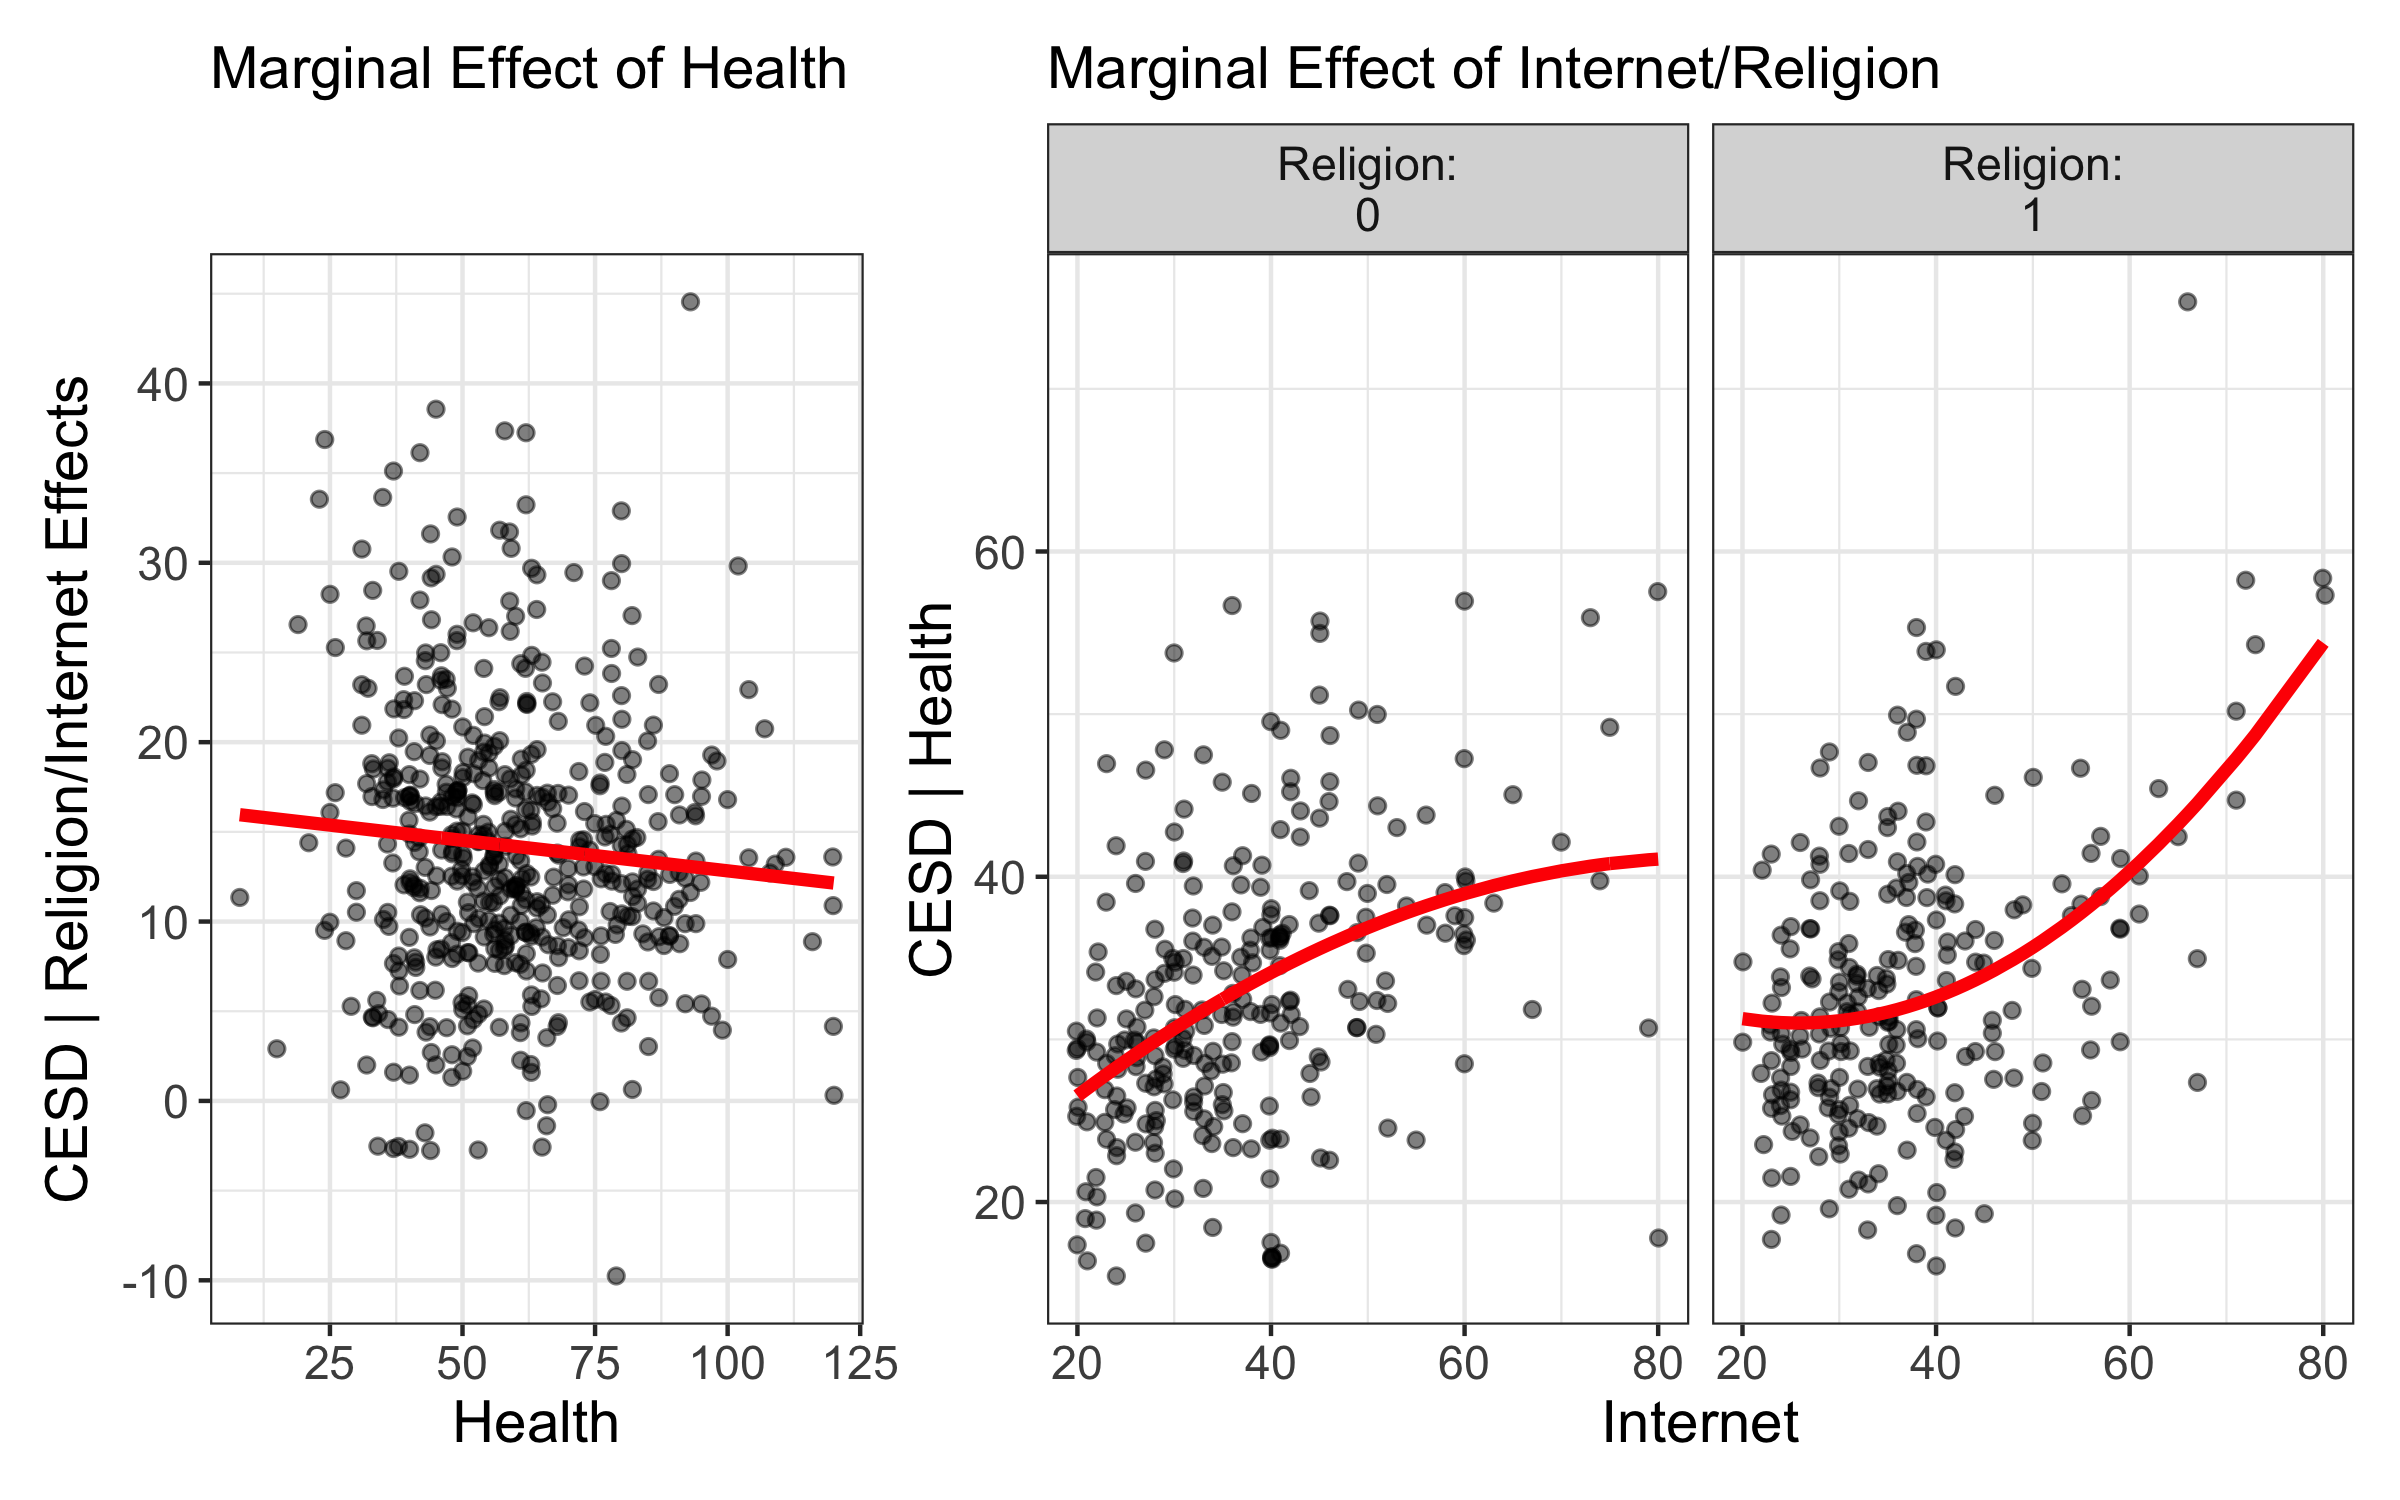
\includegraphics{visual_partitions_files/figure-latex/prpfinalexample-1} 

}

\caption{Final partial residual plots of the internet addiction model. The left plot shows the main effect of health on CESD (after controlling for BMI, age, drinking, smoking, Internet, and religion). The right plot shows the effects of Internet/rligion on CESD (after controlling for BMI, age, drinking, smoking, and health). For the labels, A = age, D = drinking, S = smoking, H = health, I = Internet, and r = religion.}\label{fig:prpfinalexample}
\end{figure}

\begin{table}[tbp]

\begin{center}
\begin{threeparttable}

\caption{\label{tab:finalmodests}ANOVA Summary Table/Effect Sizes for the Final Model.}

\begin{tabular}{llcccc}
\toprule
Variable(s) & \multicolumn{1}{c}{Effect} & \multicolumn{1}{c}{Estimate} & \multicolumn{1}{c}{SE} & \multicolumn{1}{c}{Beta} & \multicolumn{1}{c}{Semi-Partial}\\
\midrule
(Intercept) &  & -3.57 & 7.00 & 0.00 & \\
Age &  & 0.17 & 0.27 & 0.03 & 1e-04\\
BMI &  & 0.10 & 0.09 & 0.05 & 0.0056\\
Smoking &  & 1.15 & 1.90 & 0.03 & 0.0027\\
Drinking &  & 3.61 & 2.02 & 0.08 & 0.0049\\
Health &  & -0.03 & 0.02 & -0.08 & 0.0118\\
Internet/Religion & Internet & 0.58 & 0.21 & 0.80 & 0.018\\
 & Religion & 20.08 & 6.56 & 1.15 & \\
 & $\text{Internet}^2$ & 0.00 & 0.00 & -0.42 & \\
 & Internet $\times$ Religion & -0.99 & 0.31 & -2.32 & \\
 & $\text{Internet}^2 \times$ Religion & 0.01 & 0.00 & 1.38 & \\
\bottomrule
\end{tabular}

\end{threeparttable}
\end{center}

\end{table}

For the sake of completeness, we also present the statistical estimates associated with the final model (see Table \ref{tab:finalmodests}). Notice we have lumped together the Internet/religion effects (including the nonlinear components), because, again, interaction effects should not be interpreted in isolation (Appelbaum \& Cramer, 1974). Together, the two variables explain about 1.18\% of the variance.

\subsection{Summary}\label{summary}

The naive results presented in Table \ref{tab:anovatab} were both routine in applied research and potentially misleading. That model suggested health, Internet addiction, and drinking have significant effects on depression. However, a deeper investigation identified potential multiplicative effects that threaten the validity of our conclusions. There is evidence to suggest the effect of Internet addiction on depression is nonlinear, and it interacts with religion in surprising and interesting ways. Our final model may be less biased, more theoretically interesting, and easier to conceptualize.

\section{Discussion}\label{discussion}

The traditional way of reporting multivariate models rely heavily on ANOVA summary tables. These tables do not indicate the nature of effects (e.g., size/direction of main effects, how variables interact). Furthermore, these tables rely on \(p\)-values, which have no probabilistic meaning in all but the most stringent of conditions.

A better approach is to utilize what we call ``visual partitions.'' Visual partitions dissect multivariate models into relatively independent visuals that can be interpreted in isolation without bias. For confirmatory research, visual partitions clearly communicate the entirety of the multivariate model. With exploratory research, a visual partitions approach (along with marginal plots and PRPs) can be used to identify hidden nonlinear effects (including interactions).

Perhaps the greatest advantage of the visual partitions approach is that it allows one to \emph{simplify} complex multivariate models; one's multivariate model can be condensed, without bias, into a handful (or less) of easy-to-understand graphics which we call ``visual partitions.'' This simplification is becoming increasingly important in the current research landscape; there's a growing mistrust of scientific results among both scientists (Baker, 2016) and laypersons (Camargo \& Grant, 2015). Visuals provide a convenient and effective solution to increasing transparency and trust of scientific results (Tay, Parrigon, Huang, \& LeBreton, 2016). In other words, visual partitions offer a convenient \emph{communication} medium that simplifies interpretation. This paper has provided tools (marginal plots, multivariate partial residual plots), strategies, and software examples. With these resources, we hope researchers will better be able to identify important effects in their models that might otherwise have been missed.

\pagebreak

\section{Getting Started with Flexplot}\label{getting-started-with-flexplot}

As of this writing, Flexplot is available through Github only. It can be installed by first installing the devtools package:

\begin{Shaded}
\begin{Highlighting}[]
\FunctionTok{install.packages}\NormalTok{(}\StringTok{"devtools"}\NormalTok{)}
\end{Highlighting}
\end{Shaded}

With \texttt{devtools} installed, Flexplot can now be installed from Github, then loaded into the R environment:

\begin{Shaded}
\begin{Highlighting}[]
\NormalTok{devtools}\SpecialCharTok{::}\FunctionTok{install\_github}\NormalTok{(}\StringTok{"dustinfife/flexplot"}\NormalTok{)}
\FunctionTok{require}\NormalTok{(flexplot)}
\end{Highlighting}
\end{Shaded}

The \texttt{flexplot} package comes pre-loaded with the suicide ideation dataset used throughout this paper. The name of the dataset is \texttt{ideation}.

To visualize a multivariate plot, we might use the \texttt{flexplot} command as follows:

\begin{Shaded}
\begin{Highlighting}[]
\NormalTok{p }\OtherTok{=} \FunctionTok{flexplot}\NormalTok{(ideation}\SpecialCharTok{\textasciitilde{}}\NormalTok{depression }\SpecialCharTok{|}\NormalTok{ friend\_ideation }\SpecialCharTok{+}\NormalTok{ stress, }\AttributeTok{data=}\NormalTok{ideation)}
\end{Highlighting}
\end{Shaded}

Notice I'm assigning the plot to an object called \texttt{p}. This makes it easier to then use marginal plots:

\begin{Shaded}
\begin{Highlighting}[]
\FunctionTok{marginal\_plot}\NormalTok{(p)}
\end{Highlighting}
\end{Shaded}

To use partial residual plots, we have to first fit a model:

\begin{Shaded}
\begin{Highlighting}[]
\NormalTok{full\_model }\OtherTok{=} \FunctionTok{lm}\NormalTok{(ideation}\SpecialCharTok{\textasciitilde{}}\NormalTok{health }\SpecialCharTok{+} 
\NormalTok{                  stress }\SpecialCharTok{+} \FunctionTok{I}\NormalTok{(stress}\SpecialCharTok{\^{}}\DecValTok{2}\NormalTok{) }\SpecialCharTok{+}
\NormalTok{                  friend\_ideation}\SpecialCharTok{*}\NormalTok{depression, }
                \AttributeTok{data=}\NormalTok{ideation)}
\end{Highlighting}
\end{Shaded}

(Note: \texttt{friend\_ideation*depression} is a shortcut for \texttt{friend\_ideation\ +\ depression\ +\ friend\_ideation:depression}).

Now we can use PRPs to visualize any of the model's relationships:

\begin{Shaded}
\begin{Highlighting}[]
\CommentTok{\# visualize the health effect}
\FunctionTok{partial\_residual\_plot}\NormalTok{(ideation}\SpecialCharTok{\textasciitilde{}}\NormalTok{health, }
                           \AttributeTok{model=}\NormalTok{full\_model,}
                           \AttributeTok{data=}\NormalTok{ideation, }
                           \AttributeTok{added\_term =} \SpecialCharTok{\textasciitilde{}}\NormalTok{health)}
\CommentTok{\# visualize the stress linear and nonlinear effects}
\FunctionTok{partial\_residual\_plot}\NormalTok{(ideation}\SpecialCharTok{\textasciitilde{}}\NormalTok{stress, }
                           \AttributeTok{model=}\NormalTok{full\_model,}
                           \AttributeTok{data=}\NormalTok{ideation, }
                           \AttributeTok{added\_term =} \SpecialCharTok{\textasciitilde{}}\NormalTok{stress }\SpecialCharTok{+} \FunctionTok{I}\NormalTok{(stress}\SpecialCharTok{\^{}}\DecValTok{2}\NormalTok{))}
\CommentTok{\# visualize the whole model without adding terms back in}
\CommentTok{\# (this is like a residual dependence plot)}
\FunctionTok{partial\_residual\_plot}\NormalTok{(ideation}\SpecialCharTok{\textasciitilde{}}\NormalTok{stress }\SpecialCharTok{+}\NormalTok{ health }\SpecialCharTok{|} 
\NormalTok{                        depression }\SpecialCharTok{+}\NormalTok{ friend\_ideation, }
                           \AttributeTok{model=}\NormalTok{full\_model,}
                           \AttributeTok{data=}\NormalTok{ideation, }
                           \AttributeTok{method=}\StringTok{"loess"}\NormalTok{)}
    \CommentTok{\# add a loess line to the plot to compare implied fit (red) }
    \CommentTok{\# with optimal fit}
\end{Highlighting}
\end{Shaded}

\pagebreak

\section*{References}\label{references}
\addcontentsline{toc}{section}{References}

\phantomsection\label{refs}
\begin{CSLReferences}{1}{0}
\bibitem[\citeproctext]{ref-Appelbaum1974}
Appelbaum, M. I., \& Cramer, E. M. (1974). {Some problems in the nonorthogonal analysis of variance.} \emph{Psychological Bulletin}, \emph{81}(6), 335.

\bibitem[\citeproctext]{ref-Baker2016a}
Baker, M. (2016). 1,500 scientists lift the lid on reproducibility. \emph{Nature}, \emph{533}(7604), 452--454. \url{https://doi.org/10.1038/533452a}

\bibitem[\citeproctext]{ref-Bauer2005}
Bauer, D. J. (2005). {The role of nonlinear factor-to-indicator relationships in tests of measurement equivalence}. \emph{Psychological Methods}, \emph{10}(3), 305--316. \url{https://doi.org/10.1037/1082-989X.10.3.305}

\bibitem[\citeproctext]{ref-berry2012improving}
Berry, W. D., Golder, M., \& Milton, D. (2012). Improving tests of theories positing interaction. \emph{The Journal of Politics}, \emph{74}(3), 653--671.

\bibitem[\citeproctext]{ref-buja2009statistical}
Buja, A., Cook, D., Hofmann, H., Lawrence, M., Lee, E.-K., Swayne, D. F., \& Wickham, H. (2009). Statistical inference for exploratory data analysis and model diagnostics. \emph{Philosophical Transactions of the Royal Society A: Mathematical, Physical and Engineering Sciences}, \emph{367}(1906), 4361--4383.

\bibitem[\citeproctext]{ref-mistrustpublic}
Camargo, K., \& Grant, R. (2015). Public health, science, and policy debate: Being right is not enough. \emph{American Journal of Public Health}, \emph{105}(2), 232--235. \url{https://doi.org/10.2105/AJPH.2014.302241}

\bibitem[\citeproctext]{ref-Cleveland1993}
Cleveland, W. S. (1993). \emph{{Visualizing data}}. Summitt, NJ: Hobart Press.

\bibitem[\citeproctext]{ref-Cohen1968}
Cohen, J. (1968). {Multiple regression as a general data-analytic system}. \emph{Psychological Bulletin}, 426-----443. Retrieved from \url{http://citeseerx.ist.psu.edu/viewdoc/summary?doi=10.1.1.476.6180}

\bibitem[\citeproctext]{ref-cohen_applied_2013}
Cohen, J., Cohen, P., West, S. G., \& Aiken, L. S. (2013). \emph{{Applied multiple regression/correlation analysis for the behavioral sciences}}. New York, NY: Routledge.

\bibitem[\citeproctext]{ref-Cronbach1975}
Cronbach, L. J. (1975). \emph{{Beyond the two disciplines of scientific psychology.}} US: American Psychological Association. \url{https://doi.org/10.1037/h0076829}

\bibitem[\citeproctext]{ref-Ezekiel}
Ezekiel, M. (1924). A method of handling curvilinear correlation for any number of variables. \emph{Journal of the American Statistical Association}, \emph{19}(148), 431--453. \url{https://doi.org/10.1080/01621459.1924.10502899}

\bibitem[\citeproctext]{ref-Fife2019e}
Fife, D. A. (2020). {The Eight Steps of Data Analysis: A Graphical Framework to Promote Sound Statistical Analysis}. \emph{Perspectives on Psychological Science}, \emph{15}(4), 1054--1075. \url{https://doi.org/10.1177/1745691620917333}

\bibitem[\citeproctext]{ref-Fife2019c}
Fife, D. A. (2021). {Flexplot: Graphical-Based Data Analysis}. \emph{Psychological Methods}. \url{https://doi.org/10.1037/met0000424}

\bibitem[\citeproctext]{ref-Fife2019a}
Fife, D. A., \& Rodgers, J. L. (in press). {Understanding the Exploratory/Confirmatory Data Analysis Continuum: Moving Beyond the "Replication Crisis"}. \emph{American Psychologist}. Retrieved from \url{https://psyarxiv.com/5vfq6/}

\bibitem[\citeproctext]{ref-Finsaas2020}
Finsaas, M. C., \& Goldstein, B. L. (2020). {Do Simple Slopes Follow-Up Tests Lead Us Astray? Advancements in the Visualization and Reporting of Interactions}. \emph{Psychological Methods}, \emph{26}(1), 38--60. \url{https://doi.org/10.1037/met0000266}

\bibitem[\citeproctext]{ref-gelman2006data}
Gelman, A., \& Hill, J. (2006). \emph{Data analysis using regression and multilevel/hierarchical models}. Cambridge university press.

\bibitem[\citeproctext]{ref-JASPTeam2019}
JASP Team. (2019). \emph{{JASP (Version 0.10.2){[}Computer software{]}}}. Retrieved from \url{https://jasp-stats.org/}

\bibitem[\citeproctext]{ref-Johnson1936}
Johnson, P. O., \& Neyman, J. (1936). {Tests of certain linear hypotheses and their application to some educational problems.} \emph{Statistical Research Memoirs}, \emph{1}, 57--93.

\bibitem[\citeproctext]{ref-kutner2004applied}
Kutner, M. H., Nachtsheim, C. J., Neter, J., \& Li, W. (2004). \emph{{Applied linear statistical models}}. New York, NY: McGraw-Hill/Irwin.

\bibitem[\citeproctext]{ref-larsenMcCleary}
Larsen, W. A., \& McCleary, S. J. (1972). The use of partial residual plots in regression analysis. \emph{Technometrics}, \emph{14}(3), 781--790. \url{https://doi.org/10.1080/00401706.1972.10488966}

\bibitem[\citeproctext]{ref-McArdle2012}
McArdle, J. J. (2012). {Exploratory data mining using CART in the behavioral sciences.} In \emph{APA handbook of research methods in psychology, vol 3: Data analysis and research publication.} (pp. 405--421). American Psychological Association. \url{https://doi.org/10.1037/13621-020}

\bibitem[\citeproctext]{ref-McCabe2018}
McCabe, C. J., Kim, D. S., \& King, K. M. (2018). {Improving Present Practices in the Visual Display of Interactions}. \emph{Advances in Methods and Practices in Psychological Science}, \emph{1}(2), 147--165. \url{https://doi.org/10.1177/2515245917746792}

\bibitem[\citeproctext]{ref-otten}
Otten, J. J., Cheng, K., \& Drewnowski, A. (2015). Infographics and public policy: Using data visualization to convey complex information. \emph{Health Affairs}, \emph{34}(11), 1901--1907. \url{https://doi.org/10.1377/hlthaff.2015.0642}

\bibitem[\citeproctext]{ref-preachermargineffects}
Preacher, K. J., Curran, P. J., \& Bauer, D. J. (2006). Computational tools for probing interactions in multiple linear regression, multilevel modeling, and latent curve analysis. \emph{Journal of Educational and Behavioral Statistics}, \emph{31}(4), 437--448. \url{https://doi.org/10.3102/10769986031004437}

\bibitem[\citeproctext]{ref-rodgers_epistemology_2010}
Rodgers, J. L. (2010). {The epistemology of mathematical and statistical modeling: a quiet methodological revolution}. \emph{The American Psychologist}, \emph{65}(1), 1--12. \url{https://doi.org/10.1037/a0018326}

\bibitem[\citeproctext]{ref-Simmons2011a}
Simmons, J. P., Nelson, L. D., \& Simonsohn, U. (2011). {False-positive psychology: Undisclosed flexibility in data collection and analysis allows presenting anything as significant}. \emph{Psychological Science}, \emph{22}(11), 1359--1366.

\bibitem[\citeproctext]{ref-Tay2016a}
Tay, L., Parrigon, S., Huang, Q., \& LeBreton, J. M. (2016). {Graphical Descriptives: A Way to Improve Data Transparency and Methodological Rigor in Psychology}. \emph{Perspectives on Psychological Science}, \emph{11}(5), 692--701. \url{https://doi.org/10.1177/1745691616663875}

\bibitem[\citeproctext]{ref-Jamovi2018}
The Jamovi Project. (2019). \emph{{Jamovi (Version 0.9) {[}Computer Software{]}}}. Retrieved from \url{https://www.jamovi.org}

\bibitem[\citeproctext]{ref-Wagenmakers2012}
Wagenmakers, E.-J., Wetzels, R., Borsboom, D., Maas, H. L. J. van der, \& Kievit, R. A. (2012). {An Agenda for Purely Confirmatory Research}. \emph{Perspectives on Psychological Science}, \emph{7}(6), 632--638. \url{https://doi.org/10.1177/1745691612463078}

\bibitem[\citeproctext]{ref-yang2019relationships}
Yang, S.-Y., Fu, S.-H., Chen, K.-L., Hsieh, P.-L., \& Lin, P.-H. (2019). Relationships between depression, health-related behaviors, and internet addiction in female junior college students. \emph{PloS One}, \emph{14}(8), e0220784.

\end{CSLReferences}


\end{document}
